\section{Case Studies of Individual Sequences}
\label{sec:results/section_b}

In this section, we will look into the individual sequences to support the averaged result obtained in the earlier section. Out of 12 video samples, we observed that most of the video samples are consistent with the hypothesis on different QP such that most performance scores decrease as QP increases and the performance on the compressed sequences give the lower performances than the uncompressed sequences. However, in some video samples, the performance scores increase midway through the QP range but starts decreasing at high QP, and the performance for the compressed sequences outperform the uncompressed ones before the high QP. These exceptional outcomes were observed in Class B Cactus, Class D BlowingBubbles, Class E FourPeople, and Class E KristenAndSara. To uncover the reasoning for this, We will examine the video samples; Class D BasketballPass, Class E Johnny, Class D BlowingBubbles, and Class B Cactus as case studies. Instead of tracking all of the object classes, we limit the tracking on the Person class to analyze the difference between the two categories. The Person class is "cleaner" in result than other classes because the Person object class is more continuously present across the frames while other object classes such as Sports ball and Handbag are more discontinuous in frames. Not only Person class, we included the Potted plant object class in Class B Cactus. As different MSR did not make a significant differences from the regression analysis according to the previous section, we selected MSR = 16 out of different MSR values in the following analysis. Finally, we primarily focused on the general tracking performance of MOTA since this metric correlates the most with the human visual system according to \cite{leal-taixe_motchallenge_2015}. Since MOTA composes of FN, FP, and IDs from the equation \ref{eqn:MOTA}, we will examine each metric closely.  


\subsection{Class D BasketballPass}
We examined the result from the individual video sequence of Class D BasketballPass. This sequence consists of 7 Person objects and the occlusion occurs frequently in the video.  Figure \ref{fig:BasketballPass_0_multiplots_qp} shows all the performance scores on different QP at MSR = 16 from the video and Table \ref{tab:BasketballPass_0} shows each numerical value. 
\begin{figure}[!htbp]
  \centering
  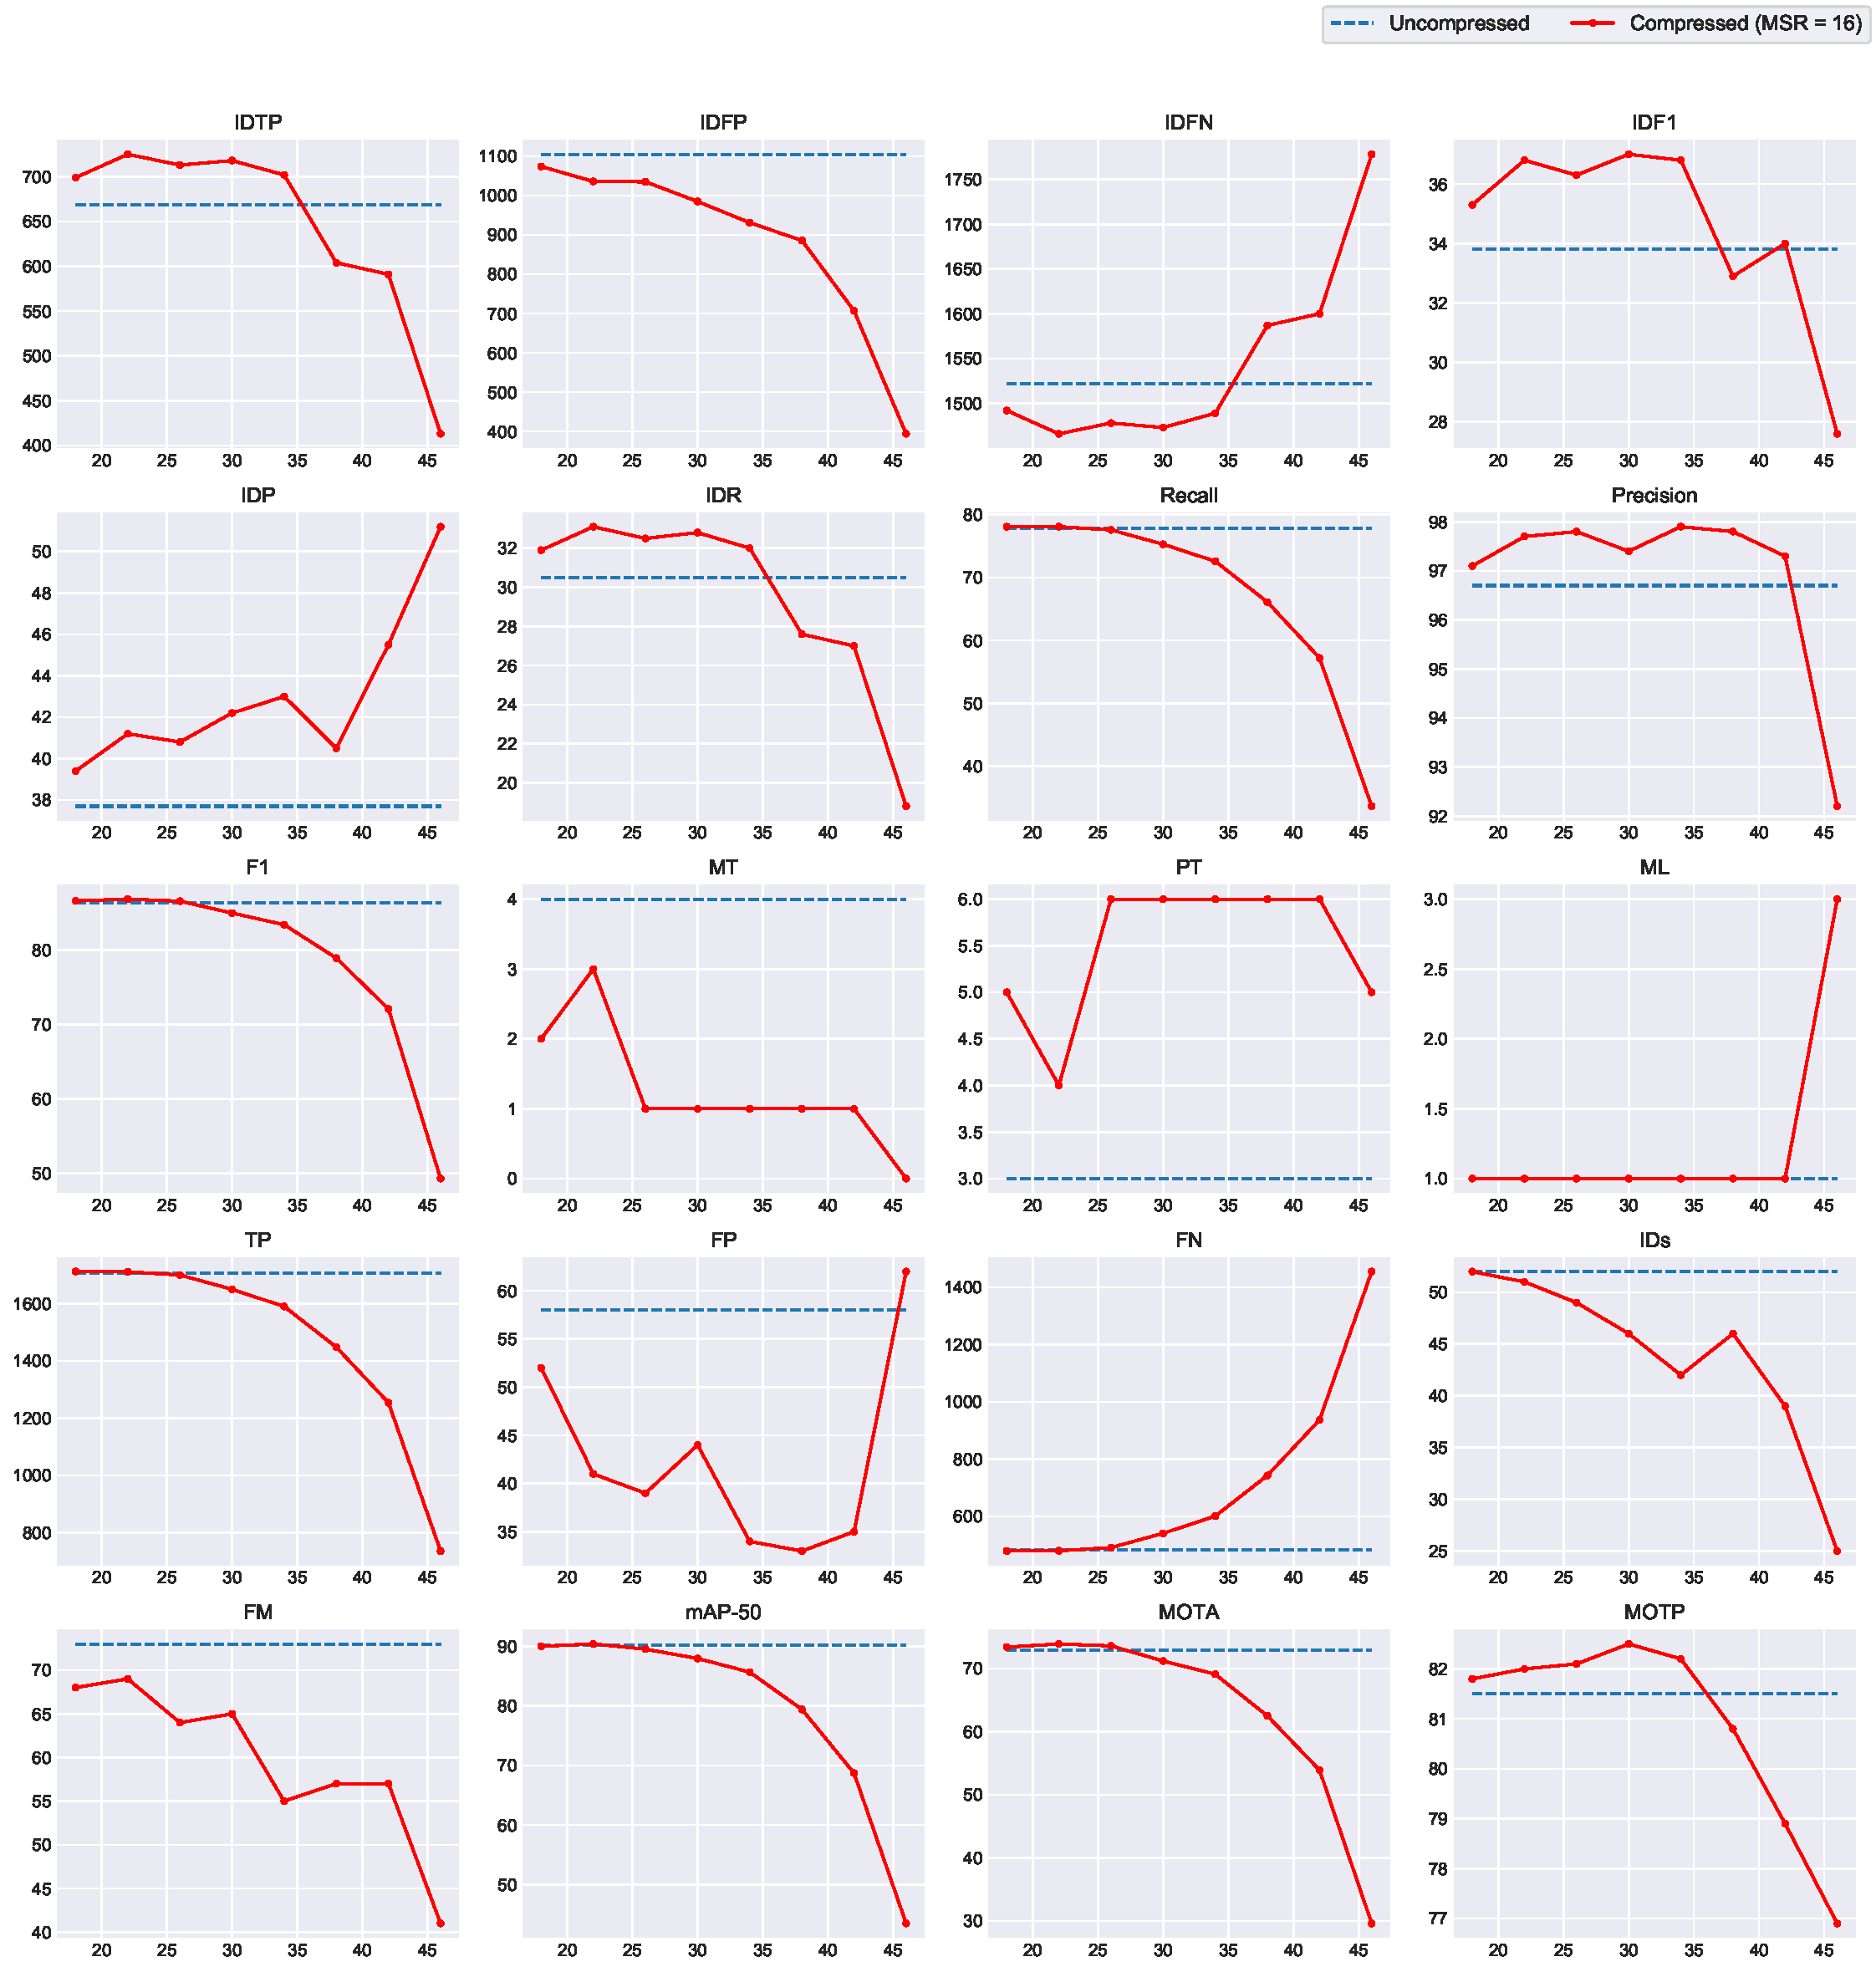
\includegraphics[width=1.0\linewidth]{img/BasketballPass_0_multiplots_qp.pdf}
  \caption[Visualization of the performance results in Class D BasketballPass at different QP for the "person" object class]
  {Visualization of the performance results in Class D BasketballPass at different QP for the "person" object class.
  }
  \label{fig:BasketballPass_0_multiplots_qp}
\end{figure}
\begin{table}[!tb]
    \centering
    \caption[Performance results on BasketballPass]
    {Performance results on BasketballPass.}
    \resizebox{1.0\linewidth}{!}{
\begin{tabular}{llrrrrrrrrrrrrrrrrrrrrr}
\toprule
          QP &          MSR &   IDTP &    IDFP &    IDFN &  IDF1 &   IDP &   IDR &  Recall &  Precision &    F1 &  GT &  MT &  PT &  ML &   TP &  FP &   FN &  IDs &  FM &  mAP-50 &  MOTA &  MOTP \\
\midrule
Uncompressed & Uncompressed & 669.00 & 1105.00 & 1522.00 & 33.80 & 37.70 & 30.50 &   77.90 &      96.70 & 86.29 &   8 &   4 &   3 &   1 & 1707 &  58 &  484 &   52 &  73 &   90.25 & 72.90 & 81.50 \\
          18 &           16 & 699.00 & 1074.00 & 1492.00 & 35.30 & 39.40 & 31.90 &   78.10 &      97.10 & 86.57 &   8 &   2 &   5 &   1 & 1712 &  52 &  479 &   52 &  68 &   90.03 & 73.40 & 81.80 \\
          22 &           16 & 725.00 & 1036.00 & 1466.00 & 36.80 & 41.20 & 33.10 &   78.10 &      97.70 & 86.81 &   8 &   3 &   4 &   1 & 1711 &  41 &  480 &   51 &  69 &   90.42 & 73.90 & 82.00 \\
          26 &           16 & 713.00 & 1035.00 & 1478.00 & 36.30 & 40.80 & 32.50 &   77.60 &      97.80 & 86.54 &   8 &   1 &   6 &   1 & 1700 &  39 &  491 &   49 &  64 &   89.54 & 73.60 & 82.10 \\
          30 &           16 & 718.00 &  985.00 & 1473.00 & 37.00 & 42.20 & 32.80 &   75.30 &      97.40 & 84.94 &   8 &   1 &   6 &   1 & 1650 &  44 &  541 &   46 &  65 &   87.98 & 71.20 & 82.50 \\
          34 &           16 & 702.00 &  931.00 & 1489.00 & 36.80 & 43.00 & 32.00 &   72.60 &      97.90 & 83.37 &   8 &   1 &   6 &   1 & 1590 &  34 &  601 &   42 &  55 &   85.69 & 69.10 & 82.20 \\
          38 &           16 & 604.00 &  886.00 & 1587.00 & 32.90 & 40.50 & 27.60 &   66.10 &      97.80 & 78.88 &   8 &   1 &   6 &   1 & 1448 &  33 &  743 &   46 &  57 &   79.42 & 62.50 & 80.80 \\
          42 &           16 & 591.00 &  707.00 & 1600.00 & 34.00 & 45.50 & 27.00 &   57.20 &      97.30 & 72.05 &   8 &   1 &   6 &   1 & 1254 &  35 &  937 &   39 &  57 &   68.72 & 53.90 & 78.90 \\
          46 &           16 & 413.00 &  394.00 & 1778.00 & 27.60 & 51.20 & 18.80 &   33.60 &      92.20 & 49.25 &   8 &   0 &   5 &   3 &  736 &  62 & 1455 &   25 &  41 &   43.45 & 29.60 & 76.90 \\
\bottomrule
\end{tabular}
    }
    \label{tab:BasketballPass_0}
\end{table}
The result is consistent with the averaged result shown in Chapter \ref{sec:results/section_a} such that the performance decreases as QP increases on most of the metrics except IDP and MOTP. To examine the result more thoroughly, we inspected the video sequence in frame by frame at different QP.
\begin{figure}[!tb]
  \centering
  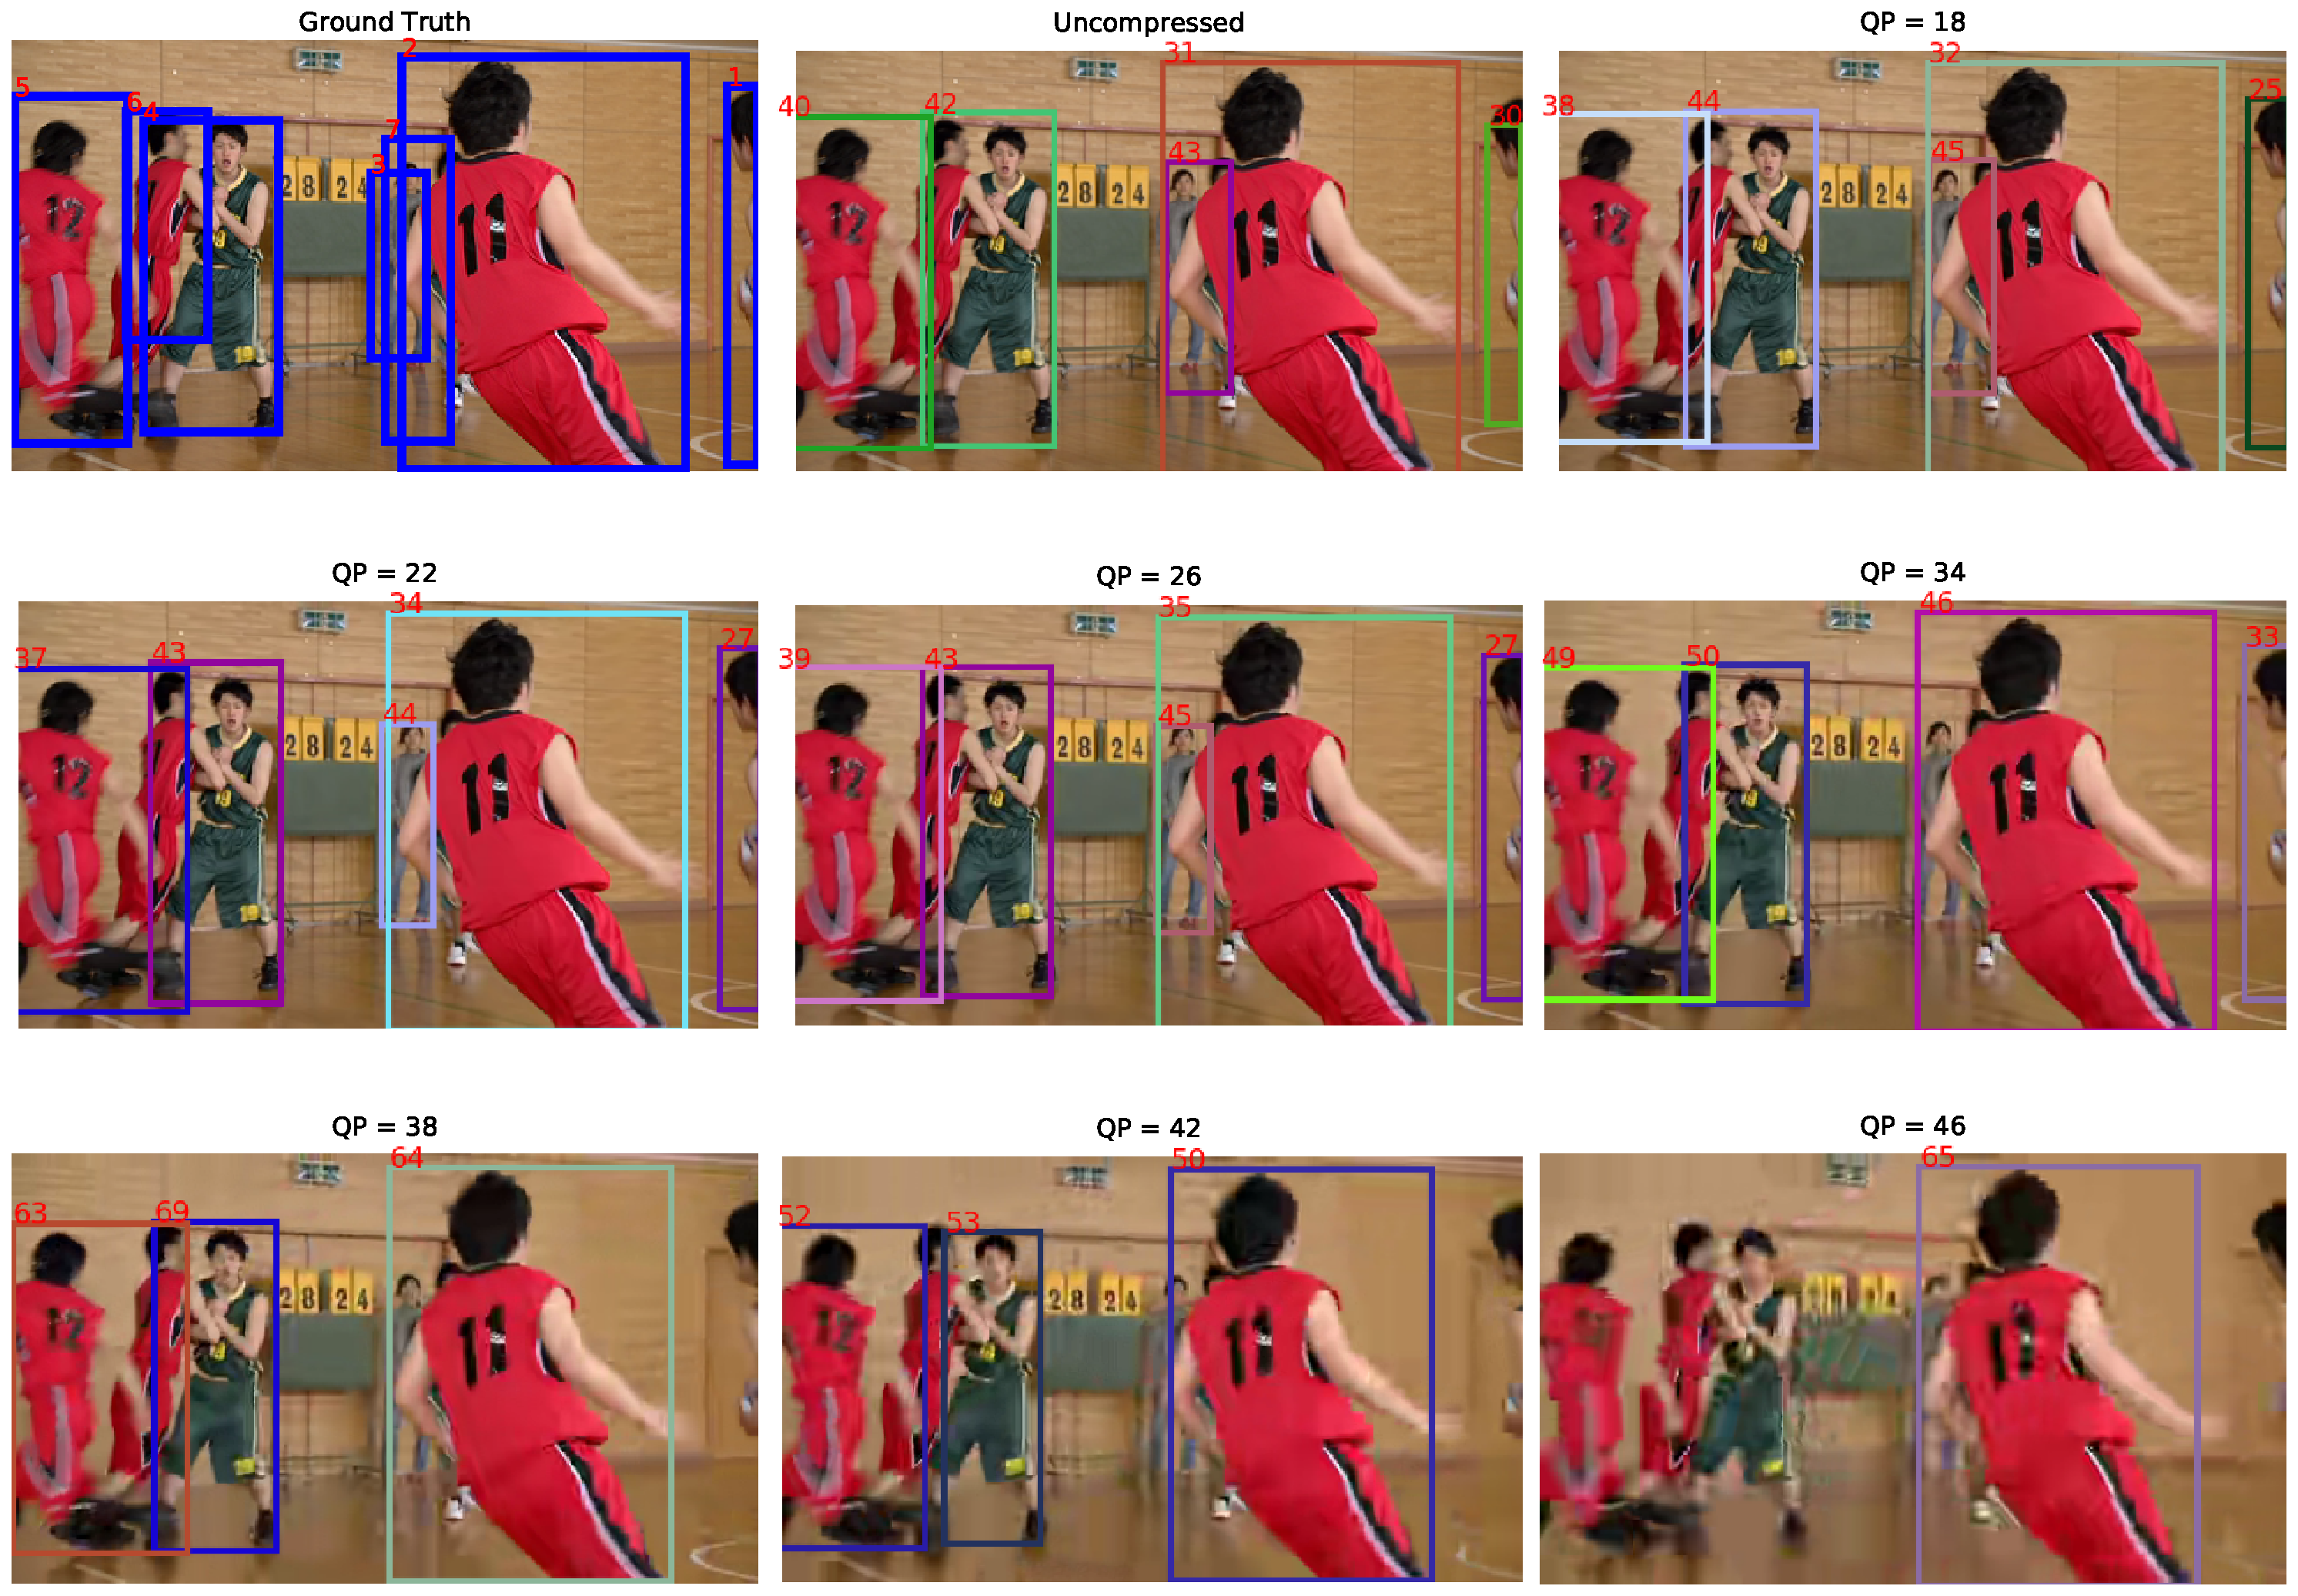
\includegraphics[width=1.0\linewidth]{img/BasketballPass_0_frame320.pdf}
  \caption[Comparison of ground truth and tracking results on the BasketballPass sequence in frames 320 at different QP]
  {
  Comparison of ground truth and tracking results on the BasketballPass sequence in frames at 320 at different QP.
  }
  \label{fig:BasketballPass_0_frame320}
\end{figure}
The figure \ref{fig:BasketballPass_0_frame320} shows comparison of ground truth, tracking results without compression, and with compression at different QP in the Class D BasketballPass sequence at frame 320 as an example. This comparison reveals that the higher the QP, the image quality decreases. As the quality decreases, the YOLO v3 detector starts failing to detect the Person objects, and hence we confirmed that FN increases. We also confirmed that IDs decreases because the number of detected objects decreases, therefore the number of times the objects being considered occluded decreases. When the detected occlusion decreases, ID switch on the trajectories should decrease since SORT does not have a feature to perform re-identification (re-ID) of the identities for the long term occlusions. The example of this situation is shown in the figure \ref{fig:BasketballPass_0_IDs}.
\begin{figure}[!tb]
  \centering
  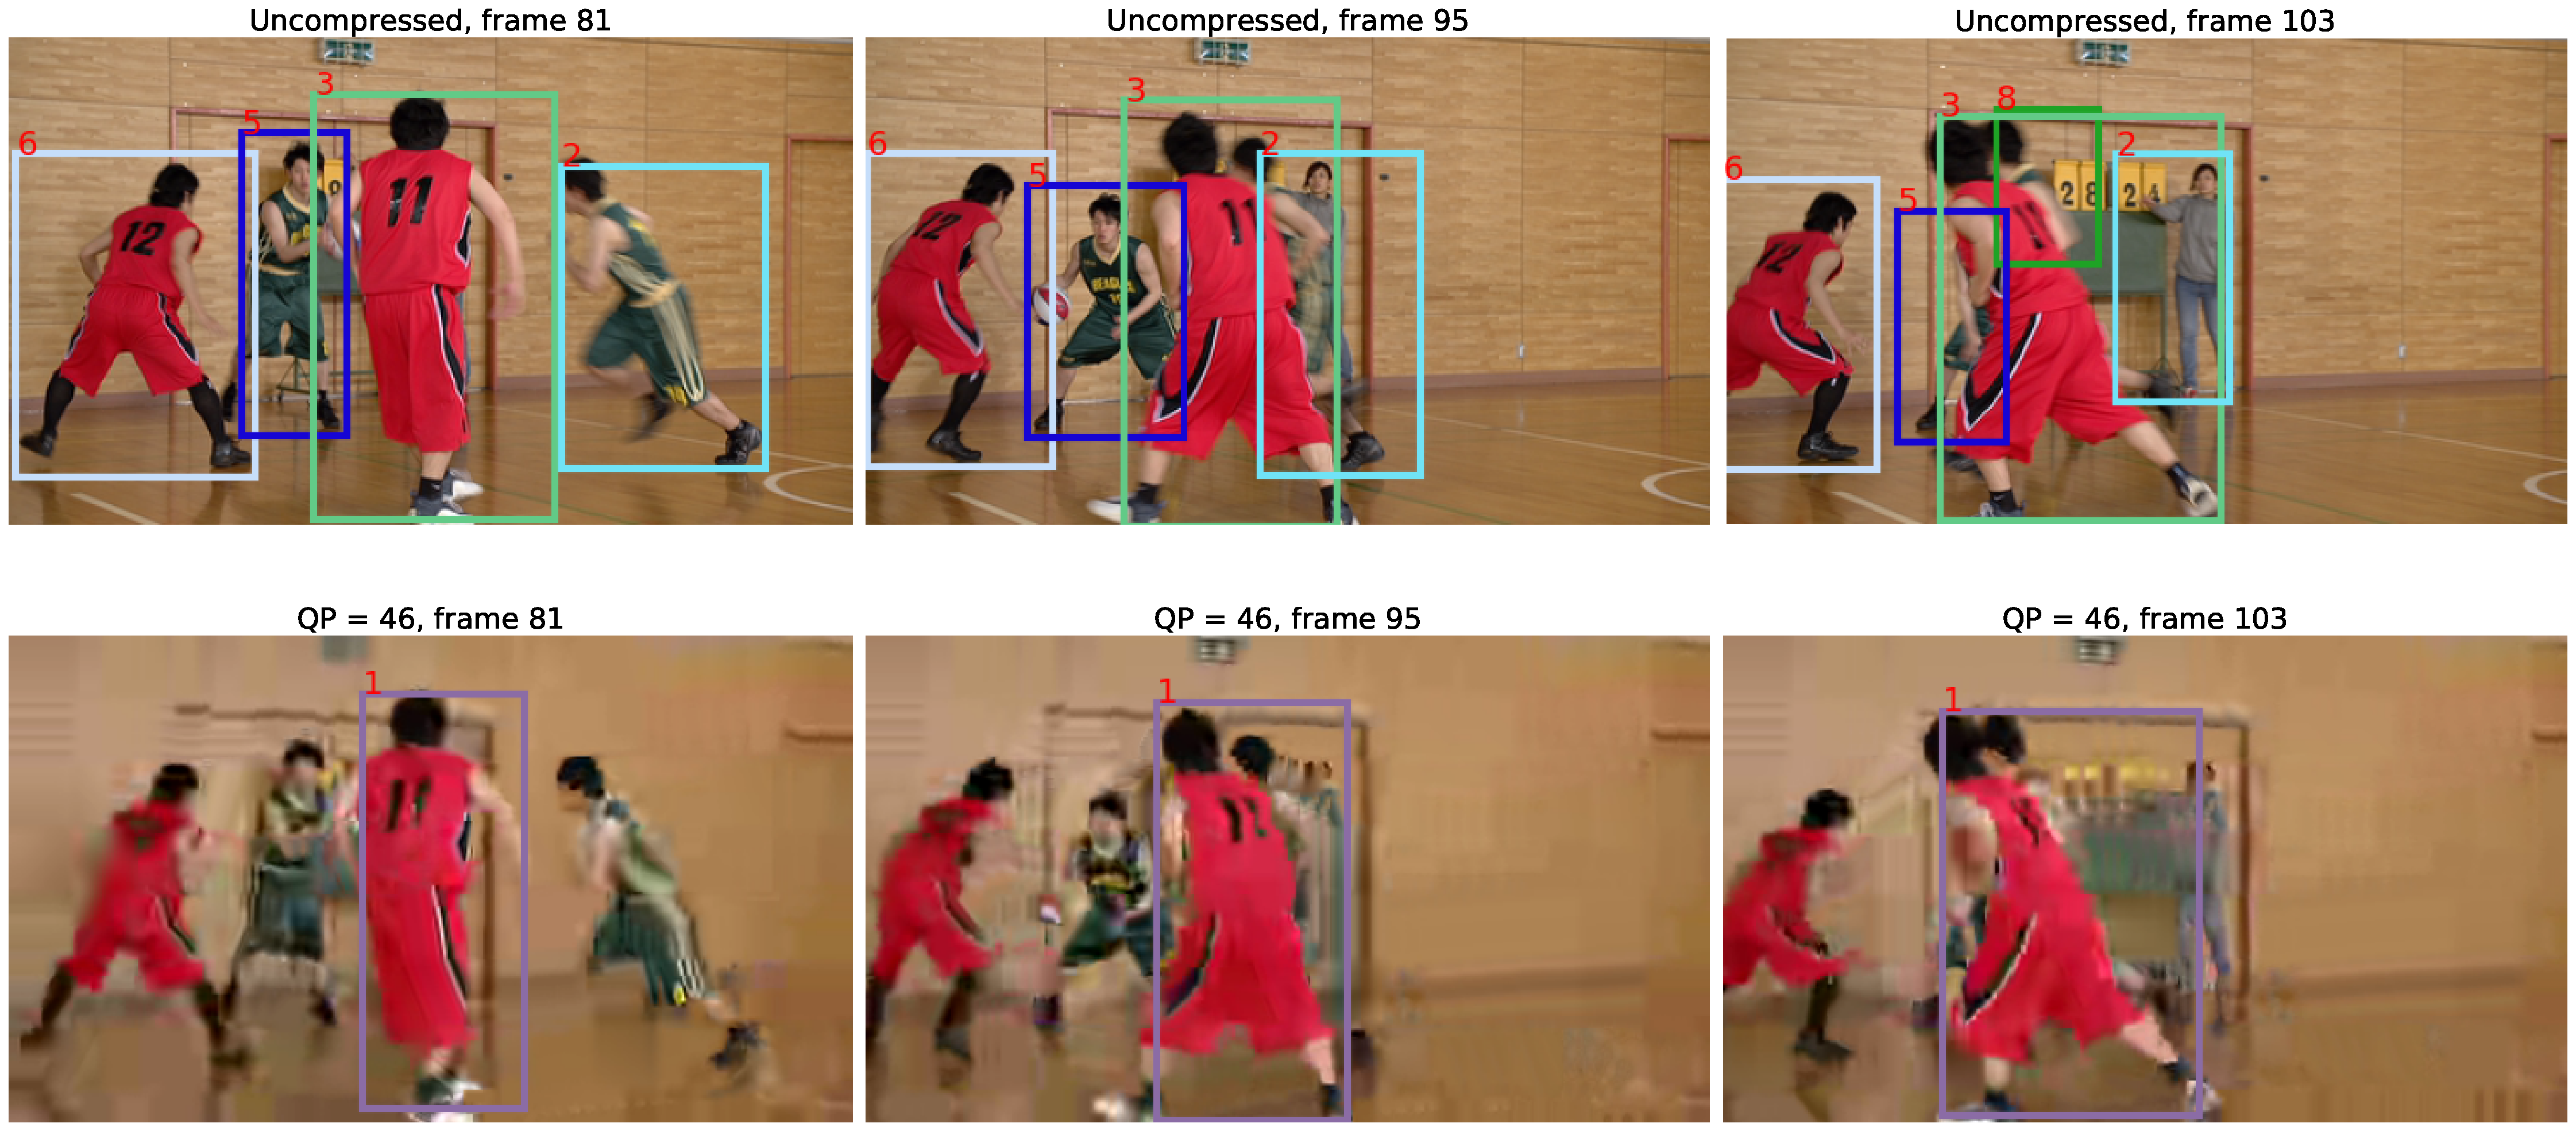
\includegraphics[width=1.0\linewidth]{img/BasketballPass_0_IDs.pdf}
  \caption[Comparison of BasketballPass frames 81, 95, 103 to explain IDs results]
  {
  Comparison of BasketballPass frames 81, 95, 103 to explain IDs results.
  }
  \label{fig:BasketballPass_0_IDs}
\end{figure}
The detected occlusion is shown in the uncompressed frames from 81 to 103 where the identities of the 2 Person objects are swapped due to the occlusions while the occlusion is not detected in the compressed frames at QP = 46. Note that re-ID was observed for the short term case. From FN, FP, and IDs, the increase of FN is significantly larger than the decrease of IDs and FP, so we concluded that MOTA decreases as QP increases based on the equation \ref{eqn:MOTA}. From the Figure \ref{fig:BasketballPass_0_multiplots_qp}, we observed that IDP increases. As we confirmed that the number of occlusions decreases as QP increases, we can verify that IDFP will decrease. Hence, based on the IDP equation \ref{eqn:IDP}, due to the drop of IDFP, IDP increases. This result can also be explained qualitatively that as QP increases, the detected occlusion occurs less, so the incorrect ID assignments occurs less, which makes ID precision higher at a higher QP.

\subsection{Class E Johnny}
Class E Johnny sequence consists of 9 Person objects. The occlusion was not observed, and the objects scarcely move. Figure \ref{fig:Johnny_0_multiplots_qp} shows the visualization of all the performance metrics at different QP, and Table \ref{tab:Johnny_0} shows the corresponding numerical values. 
\begin{figure}[!tb]
  \centering
  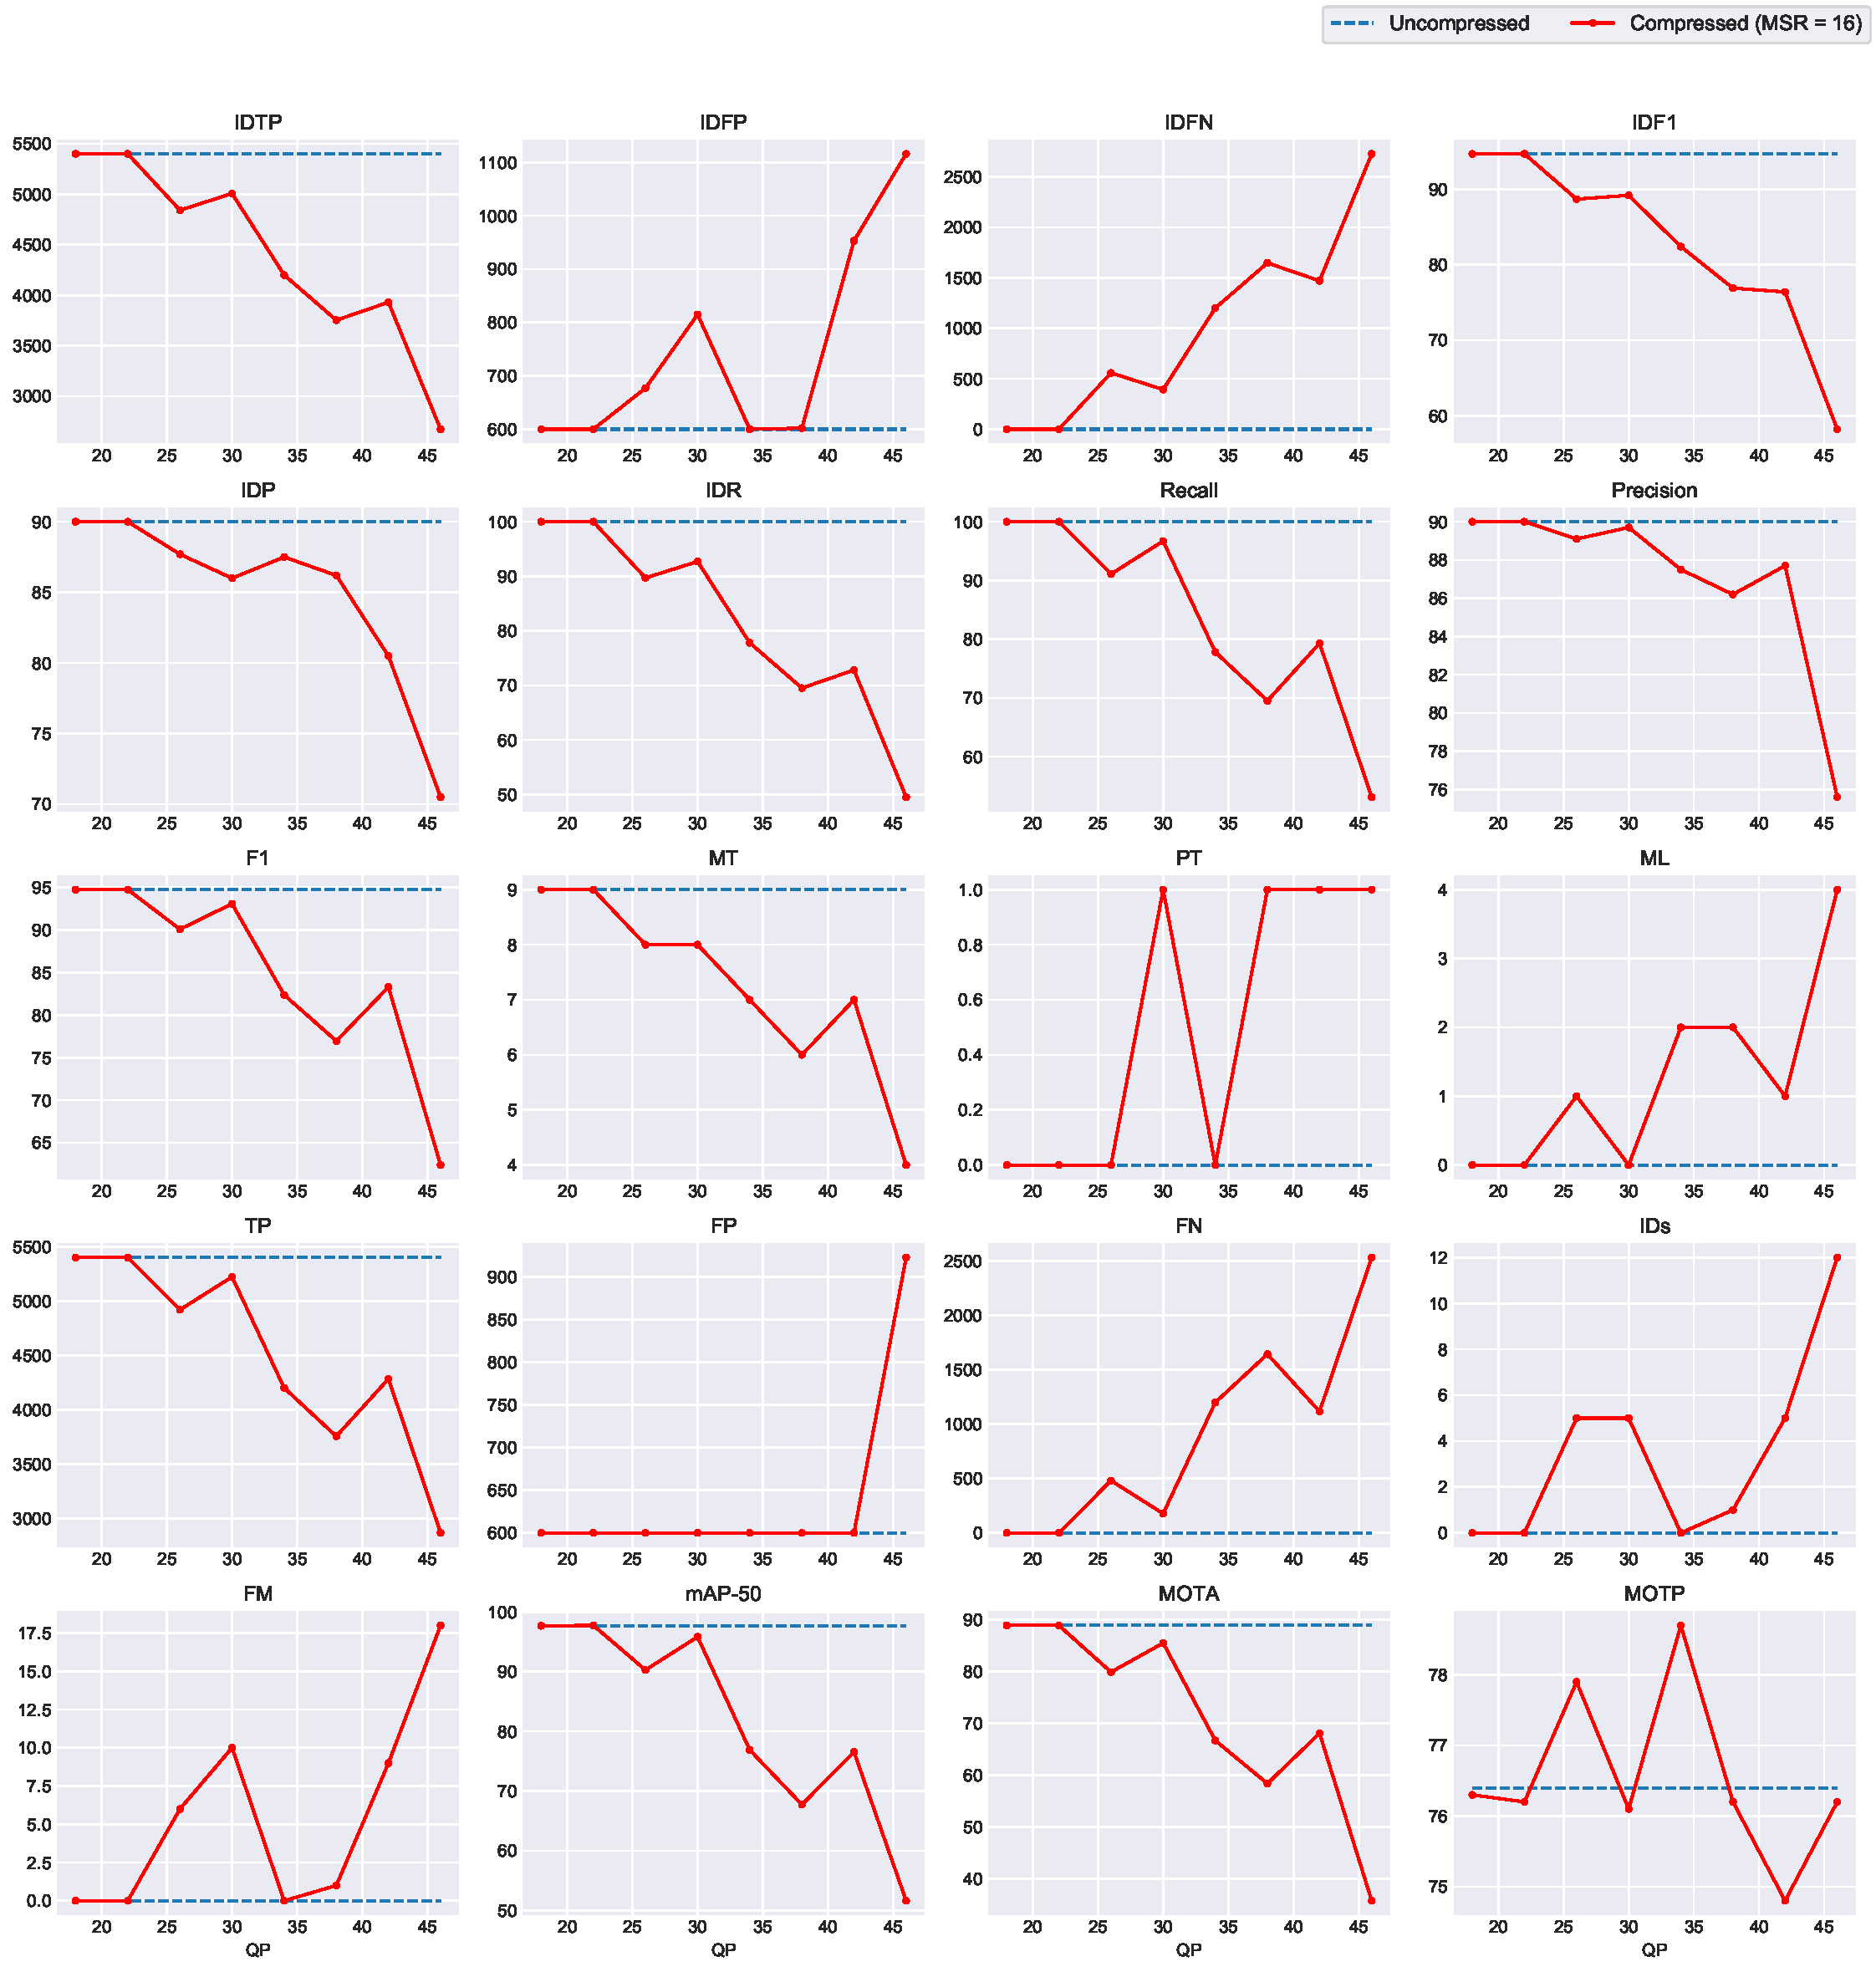
\includegraphics[width=1.0\linewidth]{img/Johnny_0_multiplots_qp.pdf}
  \caption[Visualization of the performance results on Johnny at different QP for the "person" object class]
  {
  Visualization of the performance results on Johnny at different QP for the "person" object class.
  }
  \label{fig:Johnny_0_multiplots_qp}
\end{figure}
\begin{table}[!tb]
    \centering
    \caption[Performance results on Johnny]
    {Performance results on Johnny.}
    \resizebox{1.0\linewidth}{!}{
\begin{tabular}{llrrrrrrrrrrrrrrrrrrrrr}
\toprule
          QP &          MSR &    IDTP &    IDFP &    IDFN &  IDF1 &   IDP &    IDR &  Recall &  Precision &    F1 &  GT &  MT &  PT &  ML &   TP &  FP &   FN &  IDs &  FM &  mAP-50 &  MOTA &  MOTP \\
\midrule
Uncompressed & Uncompressed & 5400.00 &  600.00 &    0.00 & 94.70 & 90.00 & 100.00 &  100.00 &      90.00 & 94.74 &   9 &   9 &   0 &   0 & 5400 & 600 &    0 &    0 &   0 &   97.72 & 88.90 & 76.40 \\
          18 &           16 & 5400.00 &  600.00 &    0.00 & 94.70 & 90.00 & 100.00 &  100.00 &      90.00 & 94.74 &   9 &   9 &   0 &   0 & 5400 & 600 &    0 &    0 &   0 &   97.70 & 88.90 & 76.30 \\
          22 &           16 & 5400.00 &  600.00 &    0.00 & 94.70 & 90.00 & 100.00 &  100.00 &      90.00 & 94.74 &   9 &   9 &   0 &   0 & 5400 & 600 &    0 &    0 &   0 &   97.76 & 88.90 & 76.20 \\
          26 &           16 & 4842.00 &  677.00 &  558.00 & 88.70 & 87.70 &  89.70 &   91.10 &      89.10 & 90.09 &   9 &   8 &   0 &   1 & 4919 & 600 &  481 &    5 &   6 &   90.29 & 79.90 & 77.90 \\
          30 &           16 & 5007.00 &  815.00 &  393.00 & 89.20 & 86.00 &  92.70 &   96.70 &      89.70 & 93.07 &   9 &   8 &   1 &   0 & 5222 & 600 &  178 &    5 &  10 &   95.85 & 85.50 & 76.10 \\
          34 &           16 & 4200.00 &  600.00 & 1200.00 & 82.40 & 87.50 &  77.80 &   77.80 &      87.50 & 82.37 &   9 &   7 &   0 &   2 & 4200 & 600 & 1200 &    0 &   0 &   76.89 & 66.70 & 78.70 \\
          38 &           16 & 3753.00 &  602.00 & 1647.00 & 76.90 & 86.20 &  69.50 &   69.50 &      86.20 & 76.95 &   9 &   6 &   1 &   2 & 3755 & 600 & 1645 &    1 &   1 &   67.73 & 58.40 & 76.20 \\
          42 &           16 & 3930.00 &  953.00 & 1470.00 & 76.40 & 80.50 &  72.80 &   79.30 &      87.70 & 83.29 &   9 &   7 &   1 &   1 & 4283 & 600 & 1117 &    5 &   9 &   76.54 & 68.10 & 74.80 \\
          46 &           16 & 2673.00 & 1116.00 & 2727.00 & 58.20 & 70.50 &  49.50 &   53.10 &      75.60 & 62.38 &   9 &   4 &   1 &   4 & 2866 & 923 & 2534 &   12 &  18 &   51.60 & 35.80 & 76.20 \\
\bottomrule
\end{tabular}
    }
    \label{tab:Johnny_0}
\end{table}
This result reveals that the most performance metrics decrease as QP increases similar to the case from the Class D BasketballPass. The decrease of performance can be verified from the Figure \ref{fig:Johnny_0_frame400} such that the objects are starting to not be detected.
\begin{figure}[!htbp]
  \centering
  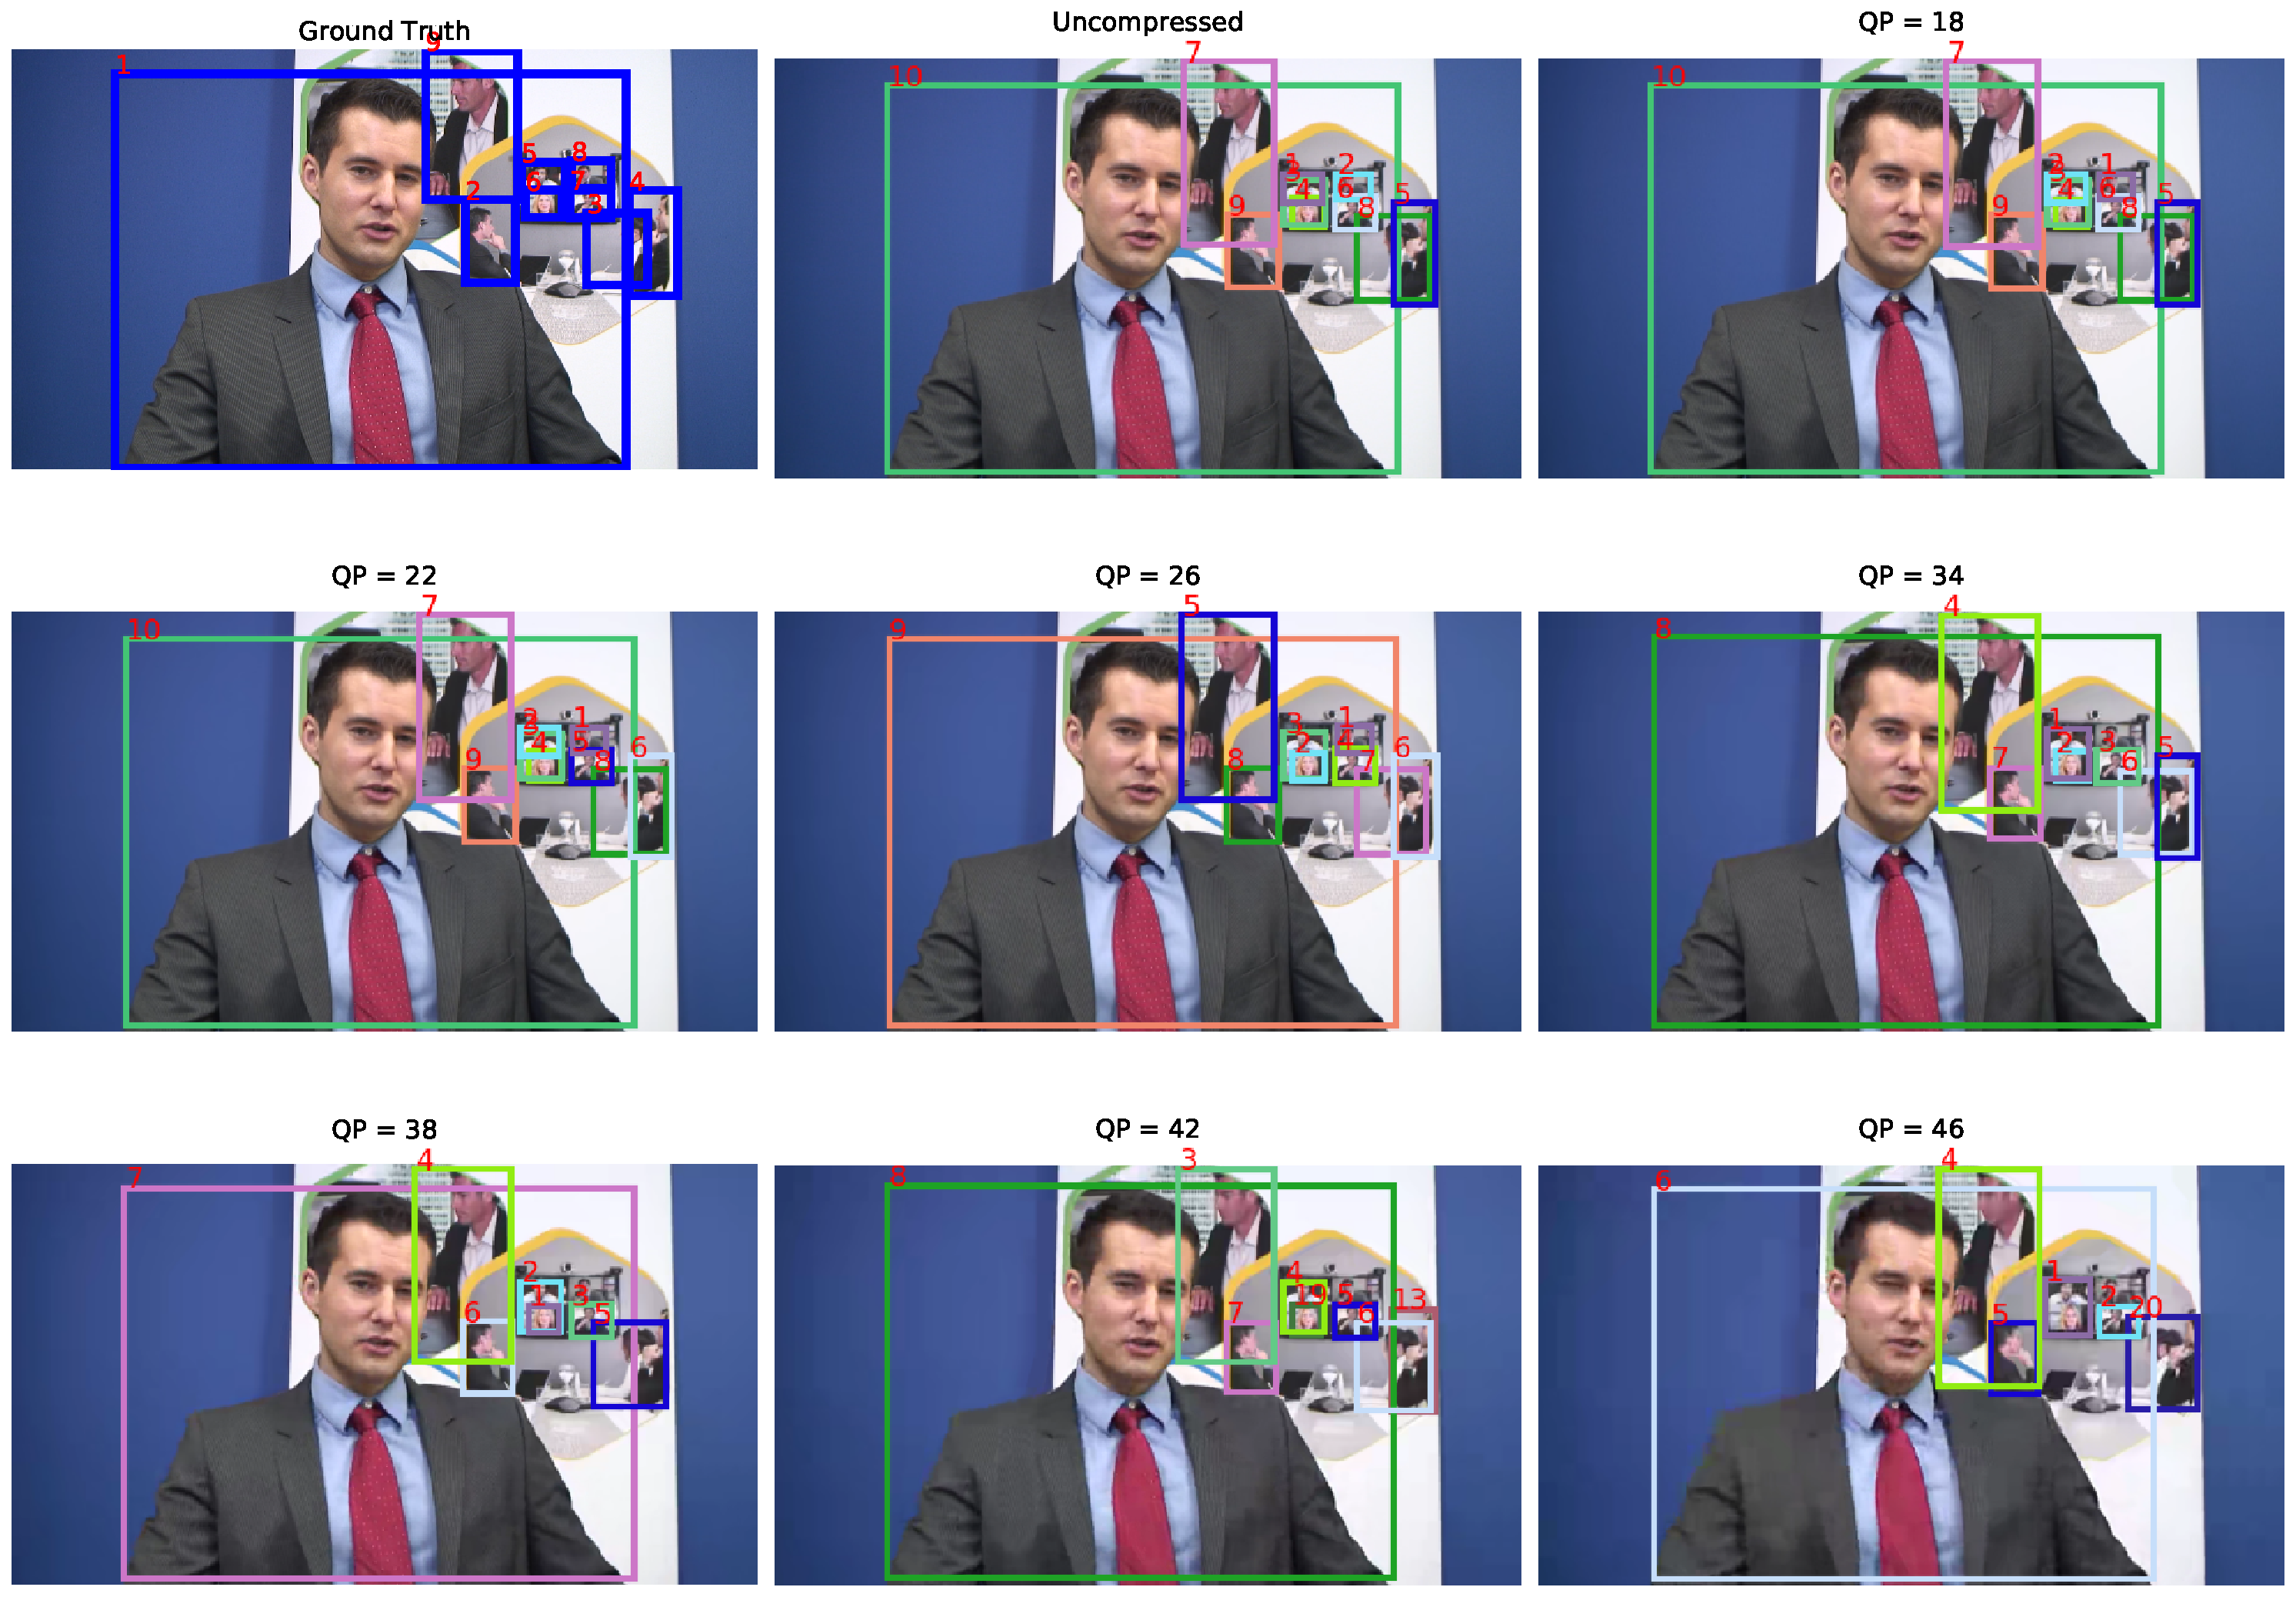
\includegraphics[width=1.0\linewidth]{img/Johnny_0_frame400.pdf}
  \caption[Comparison of Class E Johnny image frames at 320 at different QP]
  {
  Comparison of Class E Johnny image frames at 320 at different QP
  }
  \label{fig:Johnny_0_frame400}
\end{figure}
The decrease of detections proves the increase of FN. ID switch did not occur in the uncompressed sequence but was observed in the higher QP in the video sequence. Therefore, there is an increase of IDs at the higher QP. The increase of IDs can be explained qualitatively that since there is no occlusion in this sequence, ID switch between the trajectories does not occur at the lower QP but starts to occur at the high QP as the image quality drops and the different identity is assigned to the trajectory. IDs is counted whenever a different identity is assigned to the target after re-ID on the matched trajectory with the ground truth. Since the image quality drops and the detection becomes more discontinuous and re-ID is attempted but different ID is assigned to the target, IDs increases as QP increases. As an example from the figure \ref{fig:Johnny_0_IDs}, the identity of 1 Person object does not change in the uncompressed frames from 282 to 290, but change in the compressed frames at QP = 46.
\begin{figure}[!tb]
  \centering
  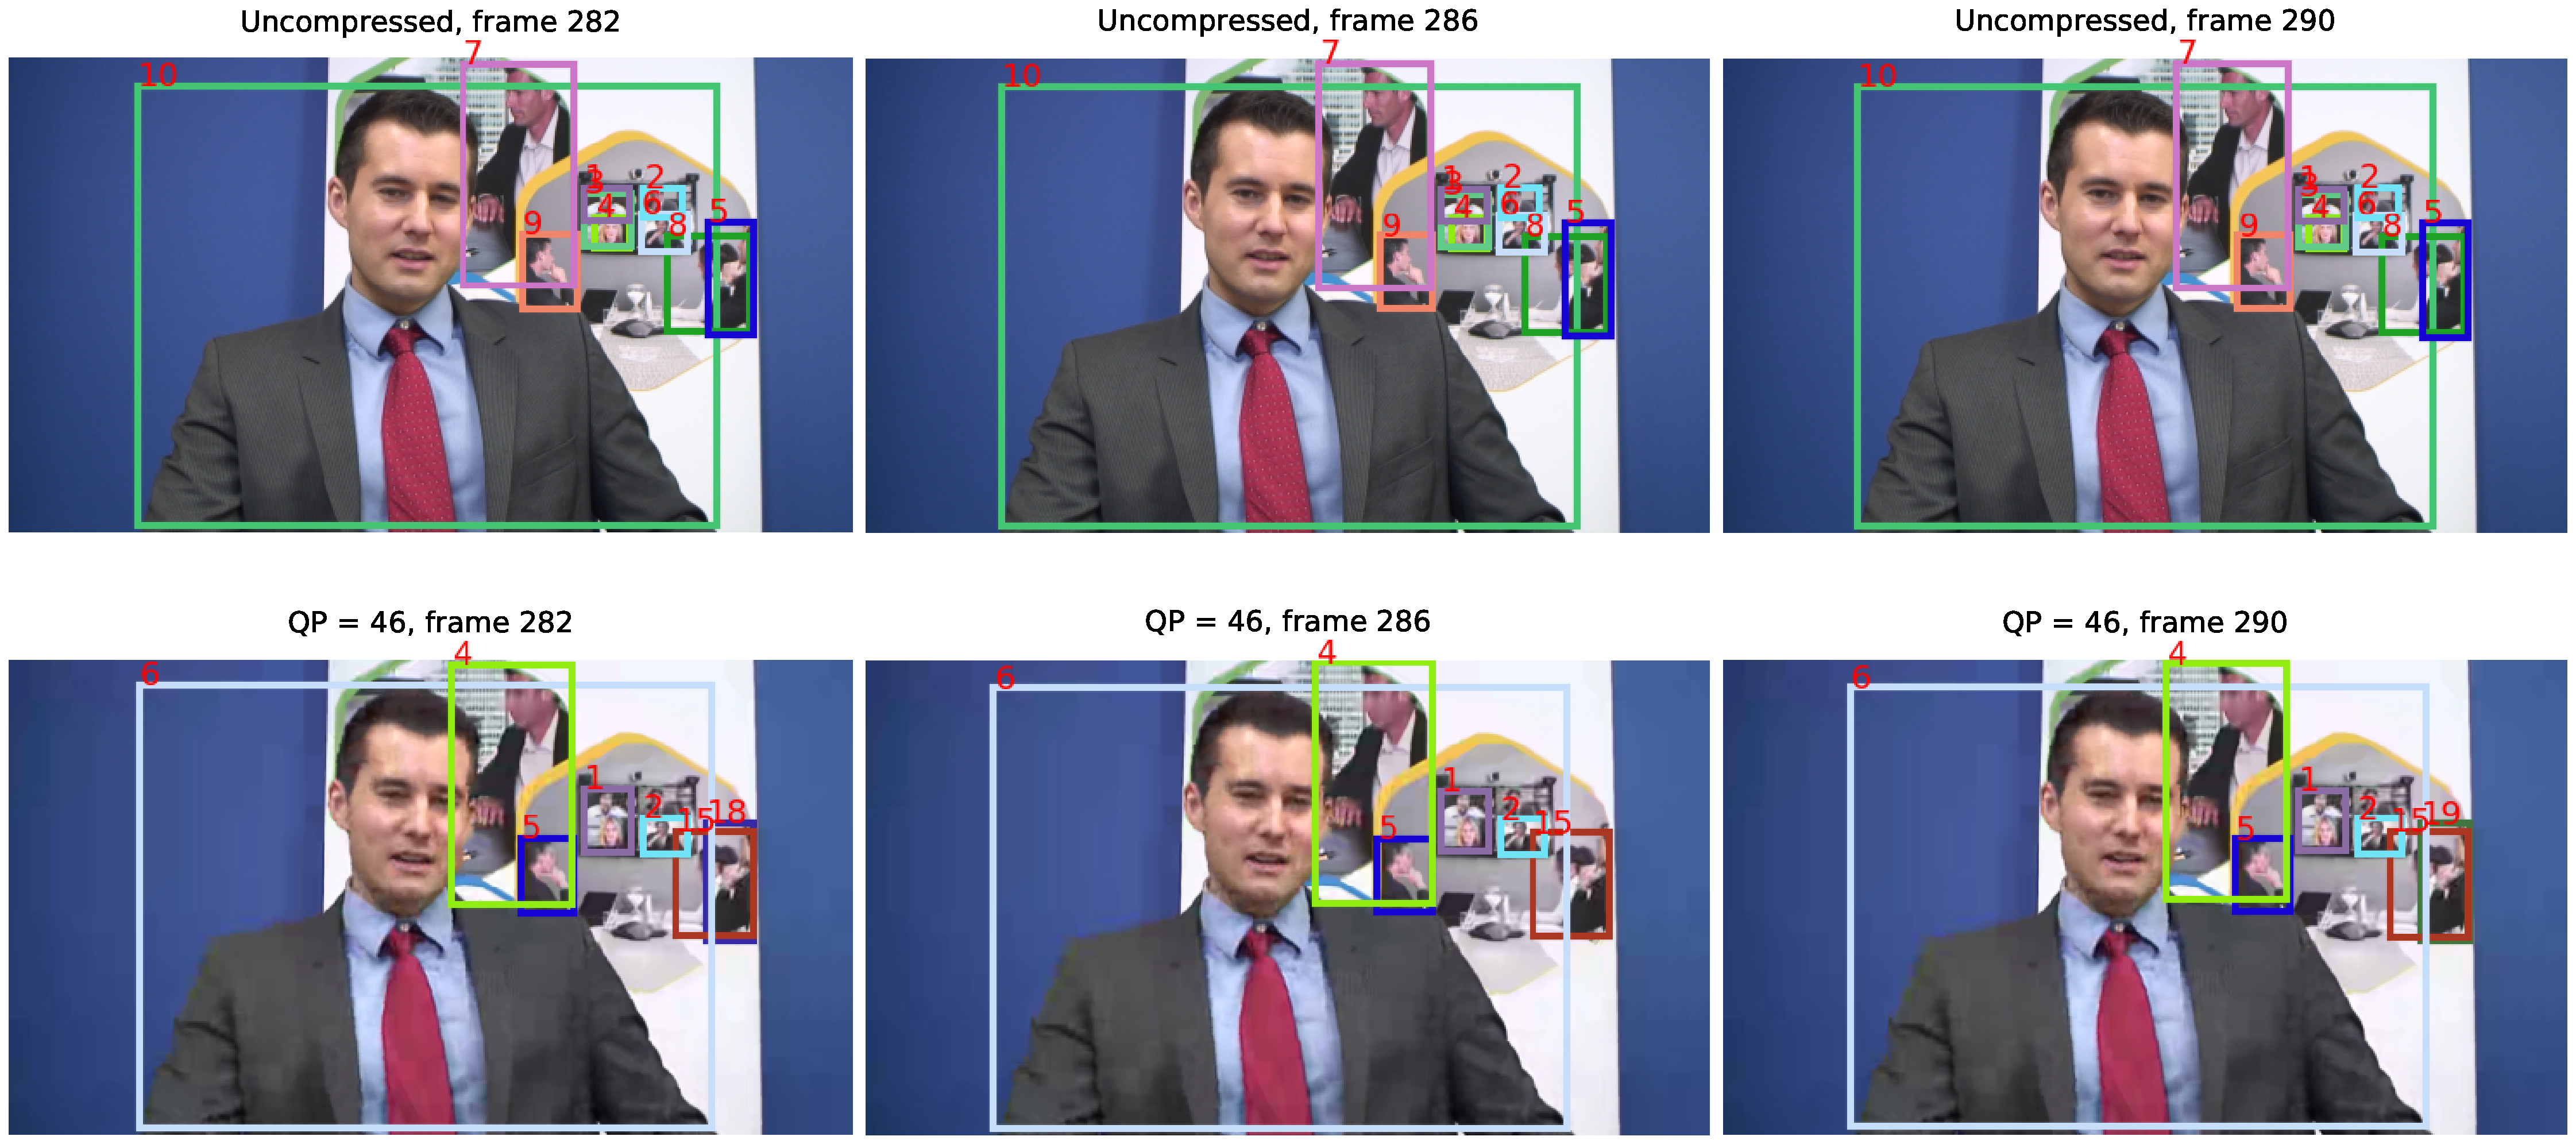
\includegraphics[width=1.0\linewidth]{img/Johnny_0_IDs.pdf}
  \caption[Comparison of Johnny frames 282, 286, 290 to explain IDs results]
  {
  Comparison of Johnny frames 282, 286, 290 to explain IDs results.
  }
  \label{fig:Johnny_0_IDs}
\end{figure}
Unlike the case from the Class D BasketballPass where the ID switch is caused by the occlusion, ID switch in this sequence is caused by the discontinuous detections. Based on all the increase of FP, FN, IDs, the general tracking performance metric of MOTA decreases as QP increases.

Since IDs increases, we expect IDP to decrease. This is because the more ID switch to occur, we expect the ID precision to be lower and indeed IDR also decreases. Therefore, we confirmed that ID performance drops as QP increases. We also observed that other metrics such as detection performance and track quality drops as QP increases. The result in this sequence is different from the result of Class D BasketballPass such that the occlusion does not occur and hence ID precision decreases as image quality drops.

\subsection{Class D BlowingBubbles}
We will now examine the sequence where we observed an increase of general tracking performance of MOTA, which can be confirmed in the visualization from Figure \ref{fig:BlowingBubbles_0_multiplots_qp} and the numerical values from Table \ref{tab:BlowingBubbles_0}.
\begin{figure}[!tb]
  \centering
  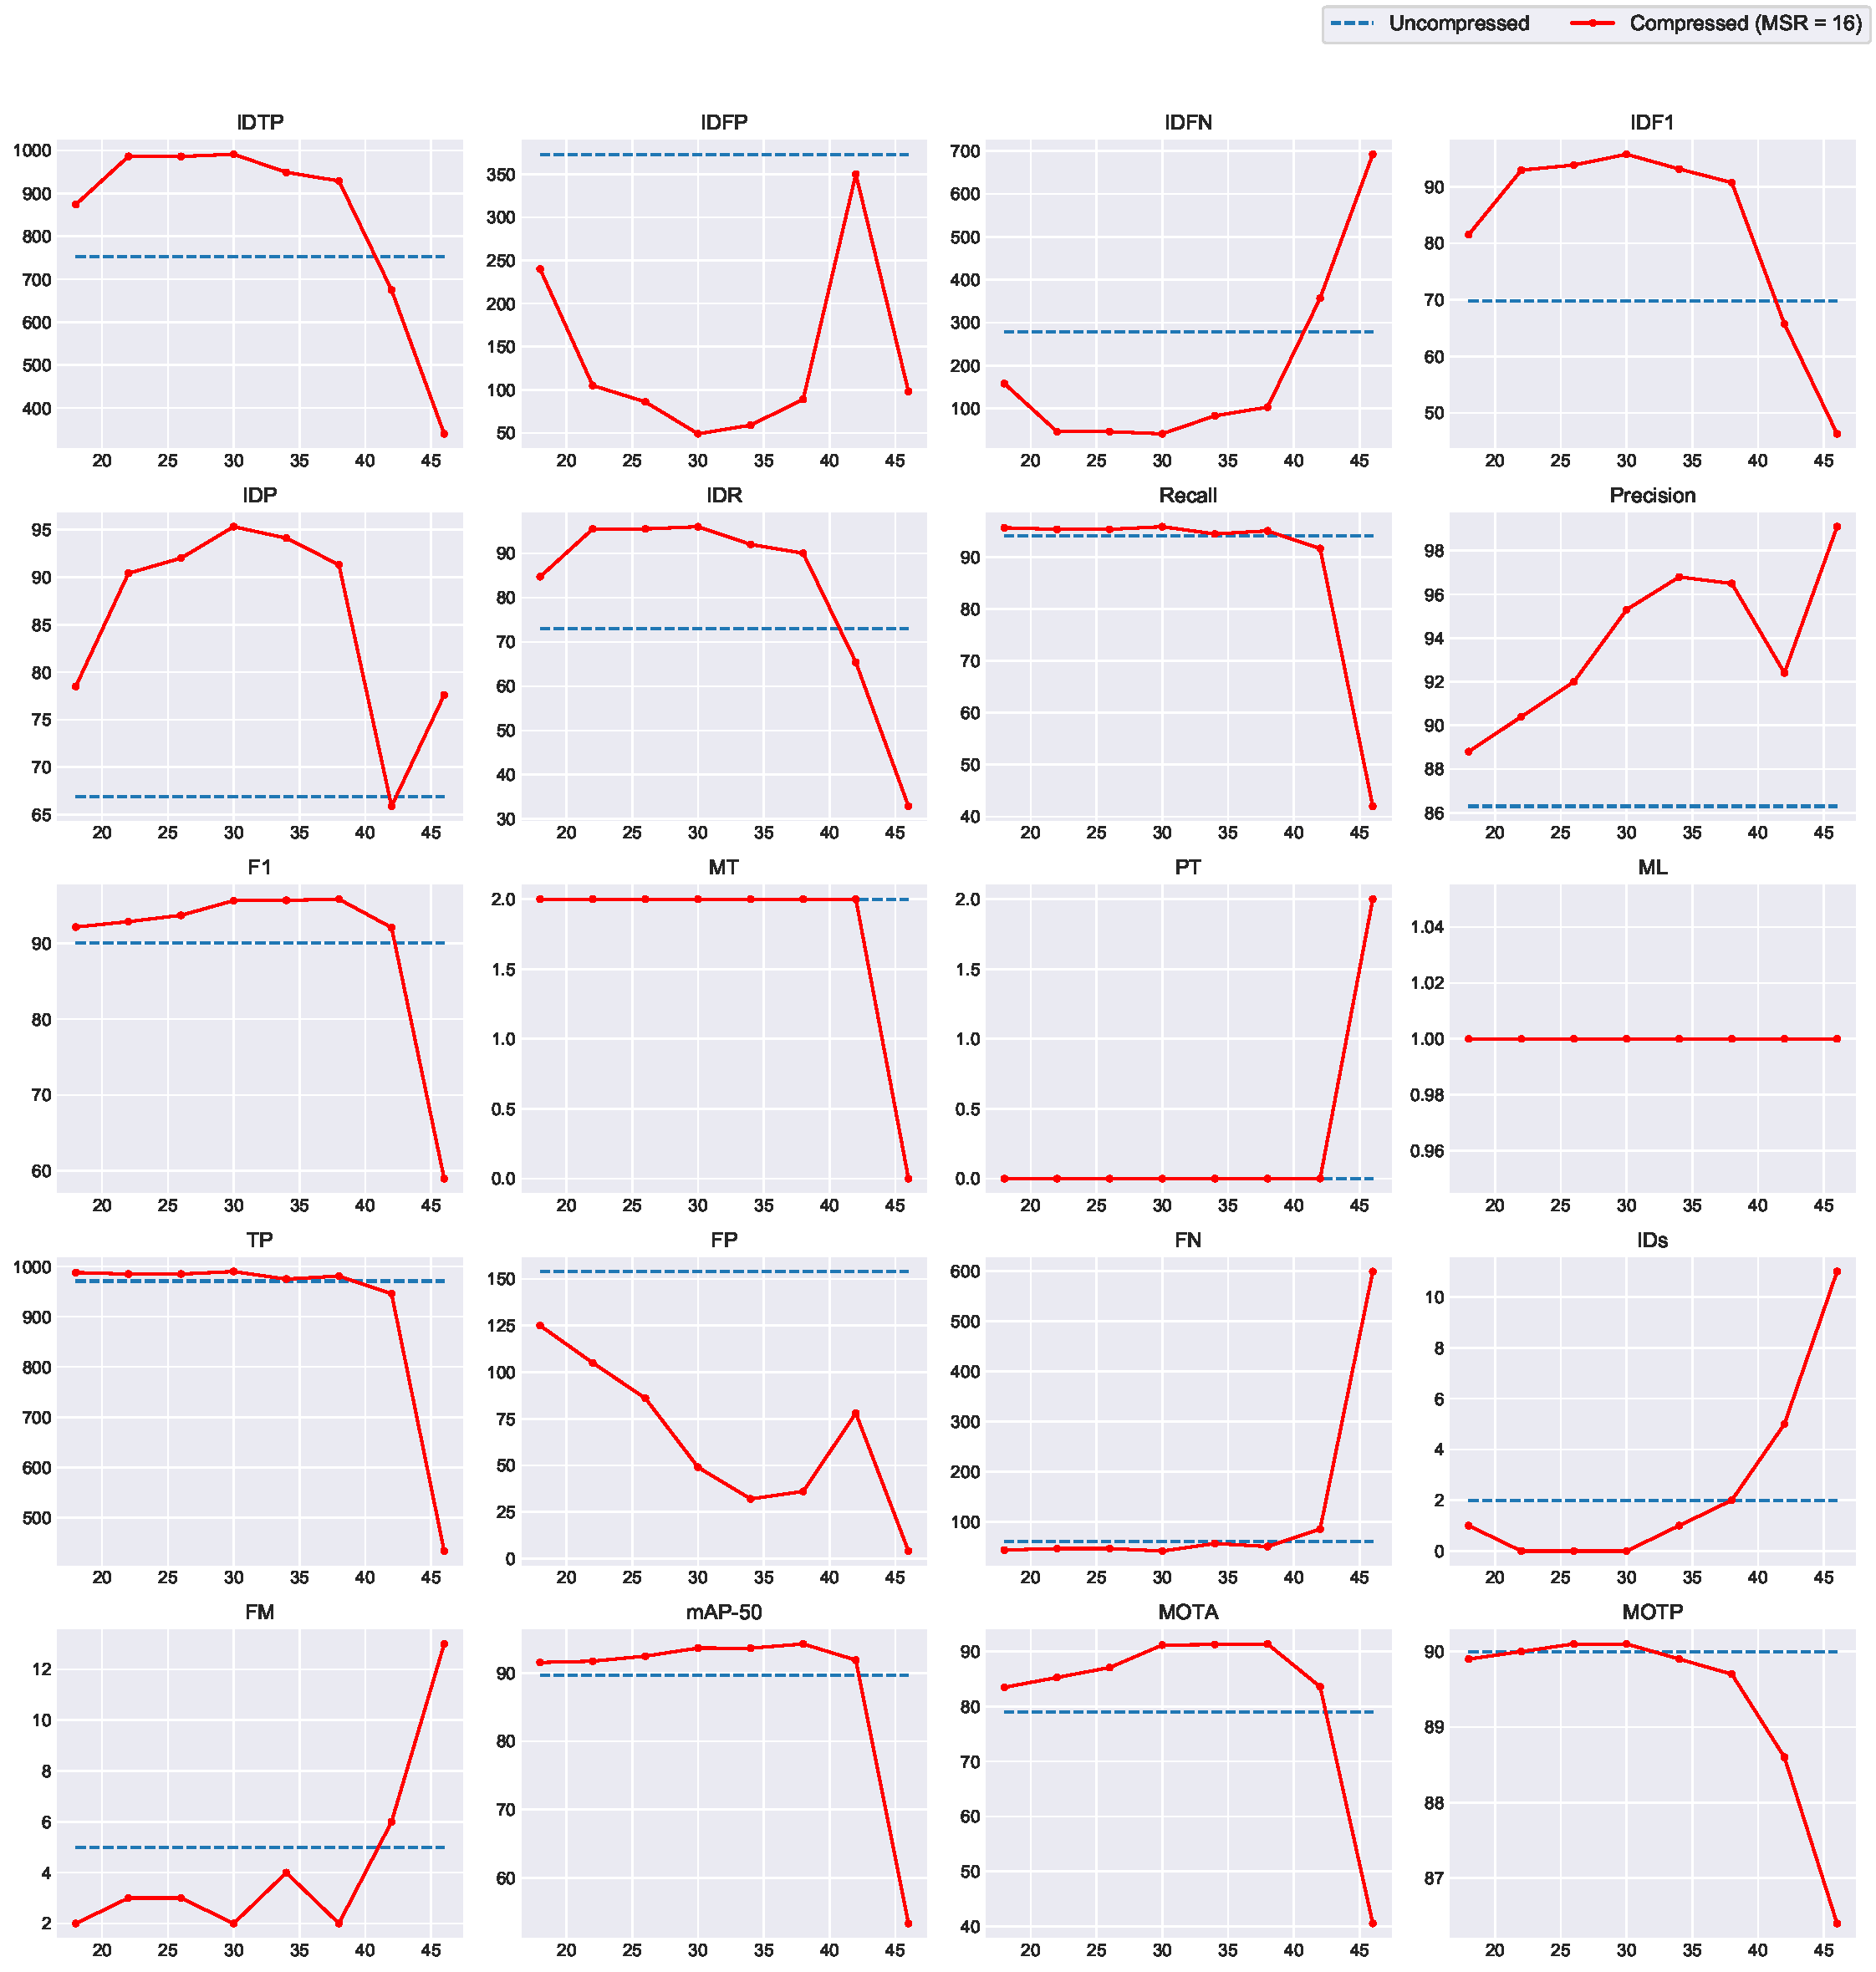
\includegraphics[width=1.0\linewidth]{img/BlowingBubbles_0_multiplots_qp.pdf}
  \caption[Visualization of the performance results on BlowingBubbles at different QP for the "person" object class]
  {
    Visualization of the performance results on BlowingBubbles at different QP for the "person" object class.
  }
  \label{fig:BlowingBubbles_0_multiplots_qp}
\end{figure}
\begin{table}[!htbp]
    \centering
    \caption[Performance results in Class D BlowingBubbles]
    {Performance results in Class D BlowingBubbles.}    \resizebox{1.0\linewidth}{!}{
    \begin{tabular}{llrrrrrrrrrrrrrrrrrrrr}
    \toprule
              QP &          MSR &   IDTP &   IDFP &   IDFN &  IDF1 &   IDP &   IDR &  Recall &  Precision &    F1 &  GT &  MT &  PT &  ML &  TP &  FP &  FN &  IDs &  FM &  MOTA &  MOTP \\
    \midrule
    Uncompressed & Uncompressed & 753.00 & 373.00 & 279.00 & 69.80 & 66.90 & 73.00 &   94.10 &      86.30 & 90.03 &   3 &   2 &   0 &   1 & 971 & 154 &  61 &    2 &   5 & 79.00 & 90.00 \\
              18 &           16 & 874.00 & 240.00 & 158.00 & 81.50 & 78.50 & 84.70 &   95.70 &      88.80 & 92.12 &   3 &   2 &   0 &   1 & 988 & 125 &  44 &    1 &   2 & 83.50 & 89.90 \\
              22 &           16 & 986.00 & 105.00 &  46.00 & 92.90 & 90.40 & 95.50 &   95.40 &      90.40 & 92.83 &   3 &   2 &   0 &   1 & 985 & 105 &  47 &    0 &   3 & 85.30 & 90.00 \\
              26 &           16 & 986.00 &  86.00 &  46.00 & 93.80 & 92.00 & 95.50 &   95.40 &      92.00 & 93.67 &   3 &   2 &   0 &   1 & 985 &  86 &  47 &    0 &   3 & 87.10 & 90.10 \\
              30 &           16 & 991.00 &  49.00 &  41.00 & 95.70 & 95.30 & 96.00 &   95.90 &      95.30 & 95.60 &   3 &   2 &   0 &   1 & 990 &  49 &  42 &    0 &   2 & 91.20 & 90.10 \\
              34 &           16 & 949.00 &  59.00 &  83.00 & 93.10 & 94.10 & 92.00 &   94.50 &      96.80 & 95.64 &   3 &   2 &   0 &   1 & 975 &  32 &  57 &    1 &   4 & 91.30 & 89.90 \\
              38 &           16 & 929.00 &  89.00 & 103.00 & 90.70 & 91.30 & 90.00 &   95.10 &      96.50 & 95.79 &   3 &   2 &   0 &   1 & 981 &  36 &  51 &    2 &   2 & 91.40 & 89.70 \\
              42 &           16 & 675.00 & 350.00 & 357.00 & 65.70 & 65.90 & 65.40 &   91.70 &      92.40 & 92.05 &   3 &   2 &   0 &   1 & 946 &  78 &  86 &    5 &   6 & 83.60 & 88.60 \\
              46 &           16 & 340.00 &  98.00 & 692.00 & 46.30 & 77.60 & 32.90 &   42.00 &      99.10 & 59.00 &   3 &   0 &   2 &   1 & 433 &   4 & 599 &   11 &  13 & 40.50 & 86.40 \\
    \bottomrule
    \end{tabular}
    }
    \label{tab:BlowingBubbles_0}
\end{table}
The MOTA visualization plot shows that the performance increases until QP = 38 but decreases thereafter. To verify this outcome, we inspected the video carefully frame by frame. From Figure \ref{fig:BlowingBubbles_0_frame465} that shows the sequence at frame 465, we observed a toy, the humanlike object, was detected as Person at the uncompressed case and QP = 18, 22, 26 but not thereafter.
\begin{figure}[!htbp]
  \centering
  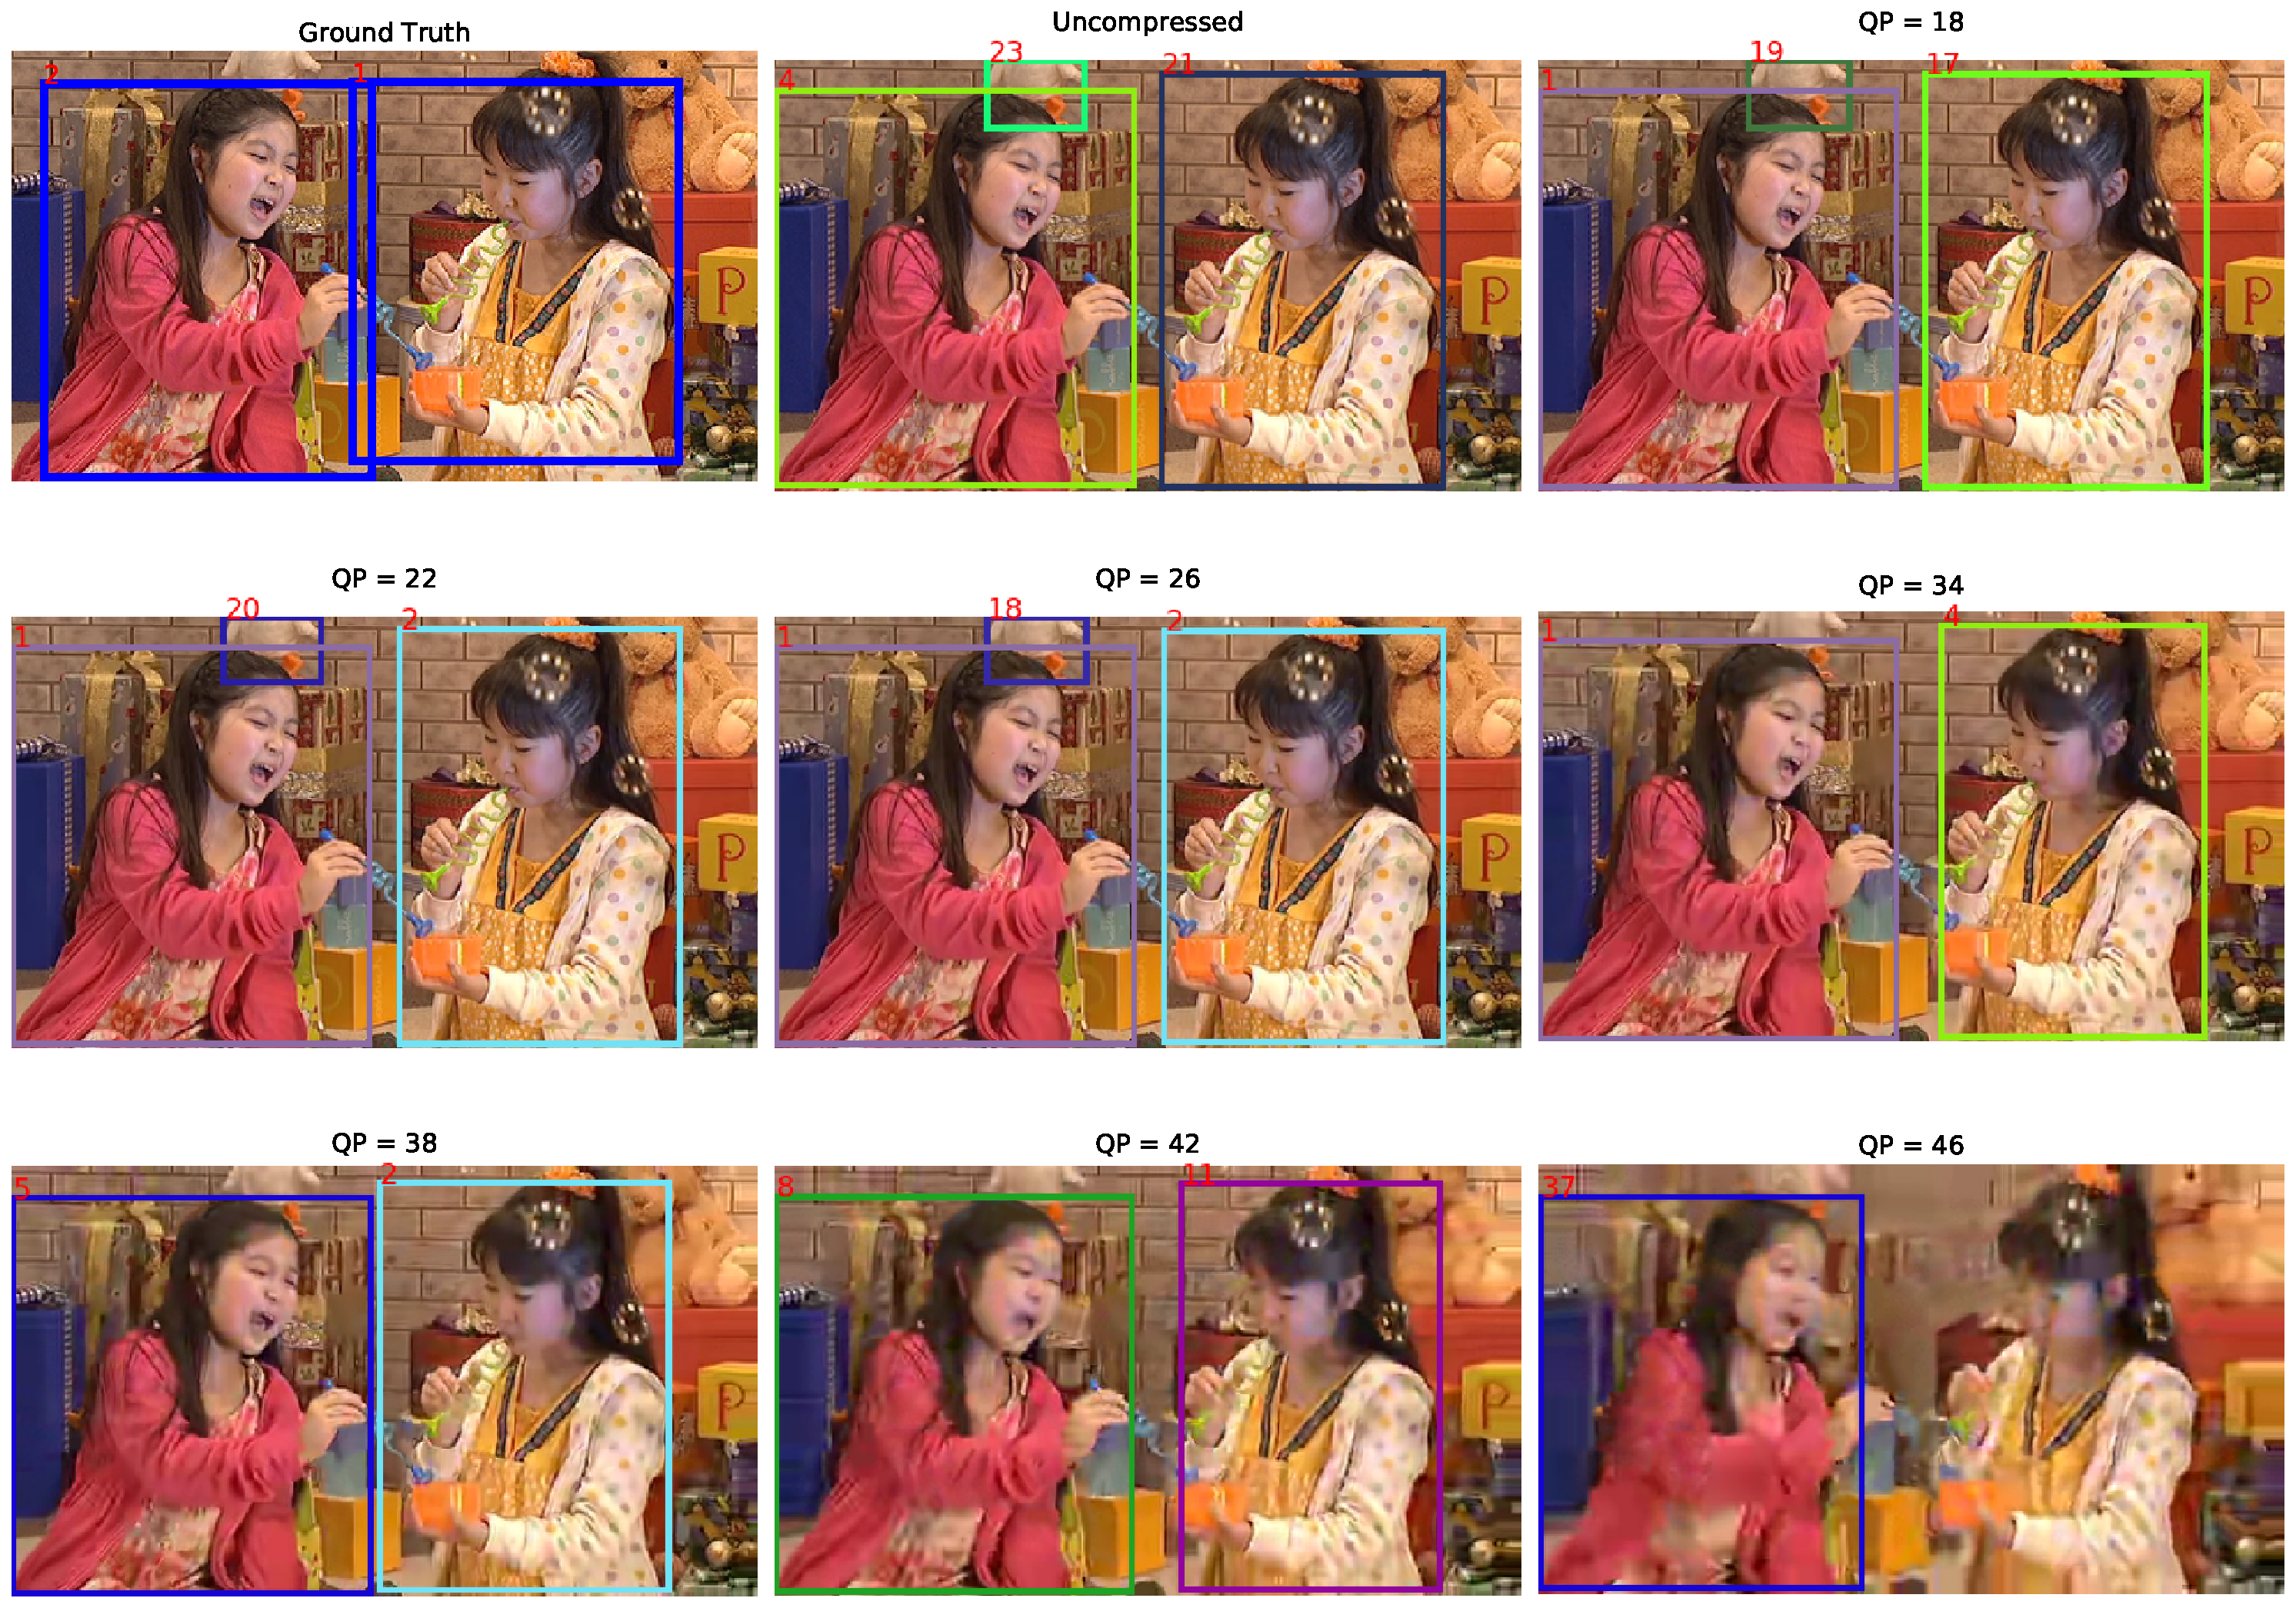
\includegraphics[width=1.0\linewidth]{img/BlowingBubbles_0_frame465.pdf}
  \caption[Comparison of Class D BlowingBubbles image frames at 465 at different QP]
  {
  Comparison of Class D BlowingBubbles image frames at 465 at different QP.
  }
  \label{fig:BlowingBubbles_0_frame465}
\end{figure}
This reveals that the detector incorrectly detect and recognize this object as Person at the lower QP, but as the image quality drops at the higher QP, the detector starts to not detect this particular object. Note that this toy object is not a part of the ground truth. This outcome was also observed in the other frames as well. This observation proves that as QP increases, FP decreases, leading to the increase of MOTA until QP = 38. After QP = 38, the image quality further drops and as can be confirmed from Figure \ref{fig:BlowingBubbles_0_frame465}, 1 Person object is not detected at QP = 46, thereby FN increases. We observed that not only MOTA, the detection performance and ID measure also result in the same way such that the performance scores increase up to the middle of QP range and decrease thereafter. For IDs, similar to the outcome in Class E Johnny, though there is no occlusion, we observed IDs to be increasing due to the drop of the image quality that makes the detection discontinuous.


\subsection{Class B Cactus}
We will illustrate the analysis result of tracking of Potted plant in this sequence. Potted plant is the only object in this video sequence. Similar to the Class D BlowingBubbles, we observed an increase of MOTA and F1 in the middle of QP range as shown in Figure \ref{fig:Cactus_58_multiplots_qp}. Table \ref{tab:Cactus_58} shows the corresponding numerical results. To confirm this result, we inspected the video sequence frame by frame and show the comparison of various QP cases at frame 32 as an example shown in Figure \ref{fig:Cactus_58_frame032}.
\begin{figure}[!htbp]
  \centering
  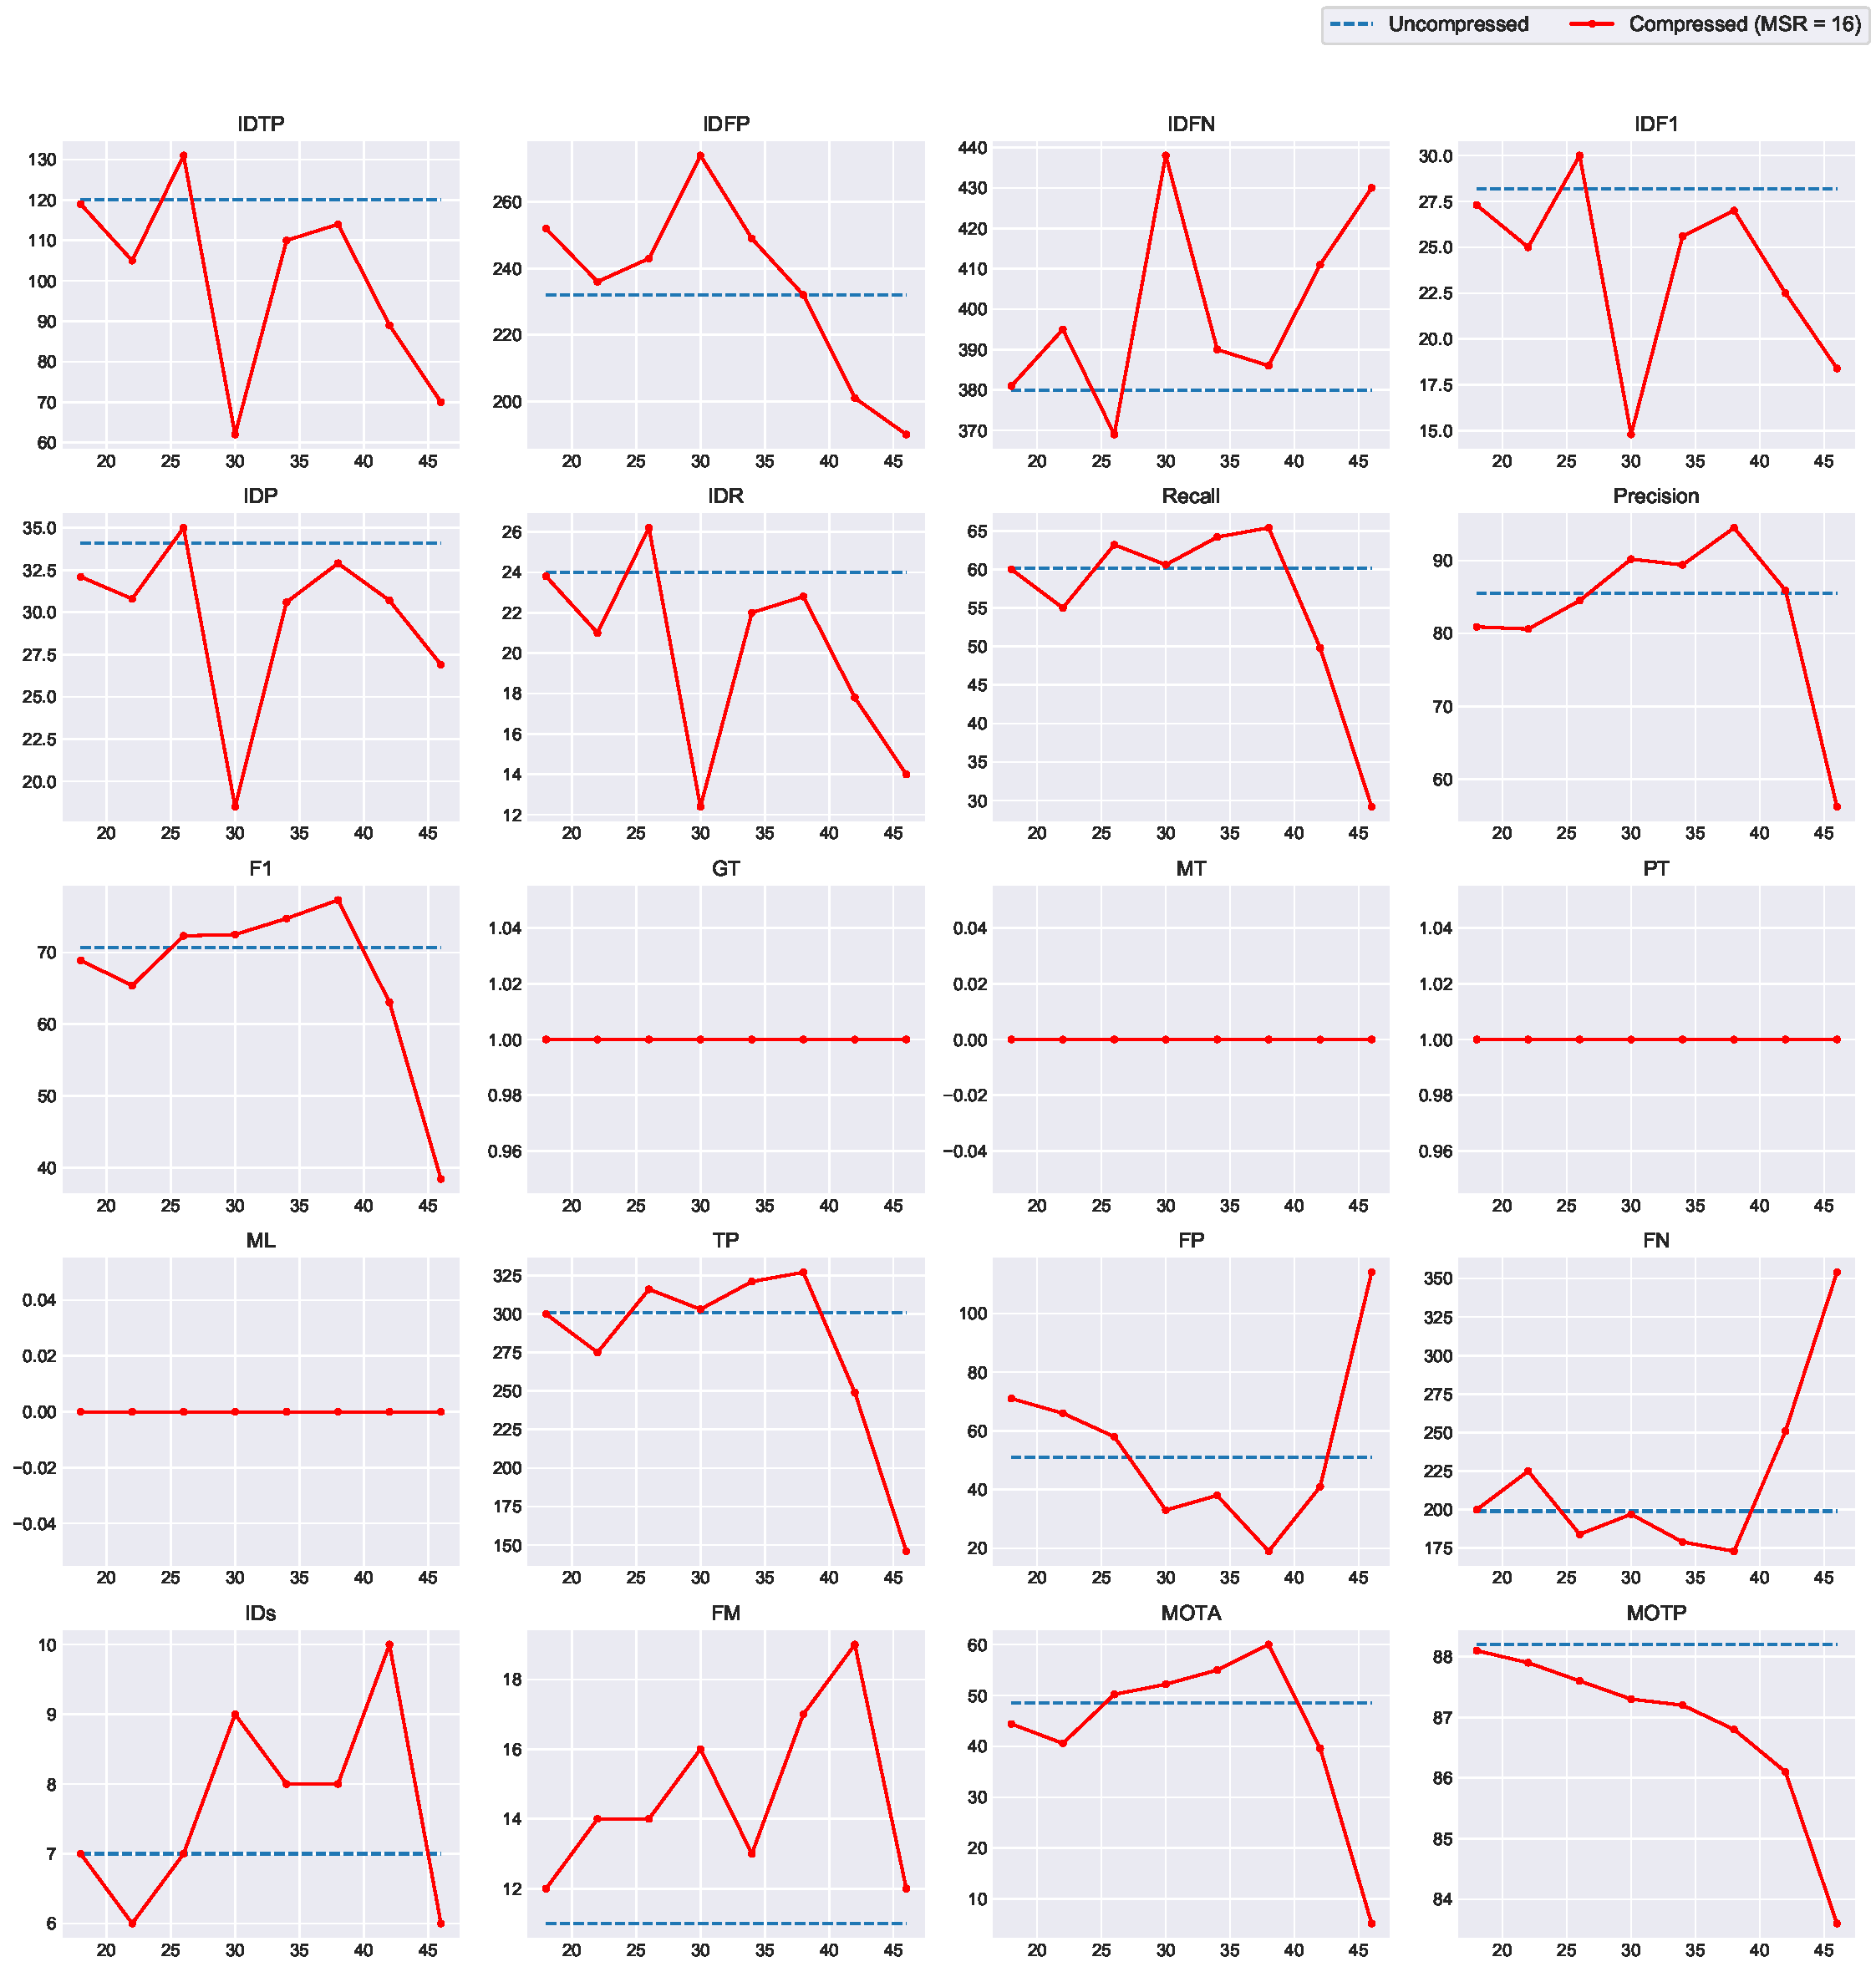
\includegraphics[width=1.0\linewidth]{img/Cactus_58_multiplots_qp.pdf}
  \caption[Visualization of the performance results in Class B Cactus at different QP]
  {
     Visualization of the performance results in Class B Cactus at different QP.
  }
  \label{fig:Cactus_58_multiplots_qp}
\end{figure}
\begin{table}[!tb]
    \centering
    \caption[Performance results on Cactus]
    {Performance results on Cactus.}
    \resizebox{1.0\linewidth}{!}{
\begin{tabular}{llrrrrrrrrrrrrrrrrrrrr}
\toprule
          QP &          MSR &   IDTP &   IDFP &   IDFN &  IDF1 &   IDP &   IDR &  Recall &  Precision &    F1 &  GT &  MT &  PT &  ML &  TP &  FP &  FN &  IDs &  FM &  MOTA &  MOTP \\
\midrule
Uncompressed & Uncompressed & 120.00 & 232.00 & 380.00 & 28.20 & 34.10 & 24.00 &   60.20 &      85.50 & 70.65 &   1 &   0 &   1 &   0 & 301 &  51 & 199 &    7 &  11 & 48.60 & 88.20 \\
          18 &           16 & 119.00 & 252.00 & 381.00 & 27.30 & 32.10 & 23.80 &   60.00 &      80.90 & 68.90 &   1 &   0 &   1 &   0 & 300 &  71 & 200 &    7 &  12 & 44.40 & 88.10 \\
          22 &           16 & 105.00 & 236.00 & 395.00 & 25.00 & 30.80 & 21.00 &   55.00 &      80.60 & 65.38 &   1 &   0 &   1 &   0 & 275 &  66 & 225 &    6 &  14 & 40.60 & 87.90 \\
          26 &           16 & 131.00 & 243.00 & 369.00 & 30.00 & 35.00 & 26.20 &   63.20 &      84.50 & 72.31 &   1 &   0 &   1 &   0 & 316 &  58 & 184 &    7 &  14 & 50.20 & 87.60 \\
          30 &           16 &  62.00 & 274.00 & 438.00 & 14.80 & 18.50 & 12.40 &   60.60 &      90.20 & 72.49 &   1 &   0 &   1 &   0 & 303 &  33 & 197 &    9 &  16 & 52.20 & 87.30 \\
          34 &           16 & 110.00 & 249.00 & 390.00 & 25.60 & 30.60 & 22.00 &   64.20 &      89.40 & 74.73 &   1 &   0 &   1 &   0 & 321 &  38 & 179 &    8 &  13 & 55.00 & 87.20 \\
          38 &           16 & 114.00 & 232.00 & 386.00 & 27.00 & 32.90 & 22.80 &   65.40 &      94.50 & 77.30 &   1 &   0 &   1 &   0 & 327 &  19 & 173 &    8 &  17 & 60.00 & 86.80 \\
          42 &           16 &  89.00 & 201.00 & 411.00 & 22.50 & 30.70 & 17.80 &   49.80 &      85.90 & 63.05 &   1 &   0 &   1 &   0 & 249 &  41 & 251 &   10 &  19 & 39.60 & 86.10 \\
          46 &           16 &  70.00 & 190.00 & 430.00 & 18.40 & 26.90 & 14.00 &   29.20 &      56.20 & 38.43 &   1 &   0 &   1 &   0 & 146 & 114 & 354 &    6 &  12 &  5.20 & 83.60 \\
\bottomrule
\end{tabular}
    }
    \label{tab:Cactus_58}
\end{table}
\begin{figure}[!htbp]
  \centering
  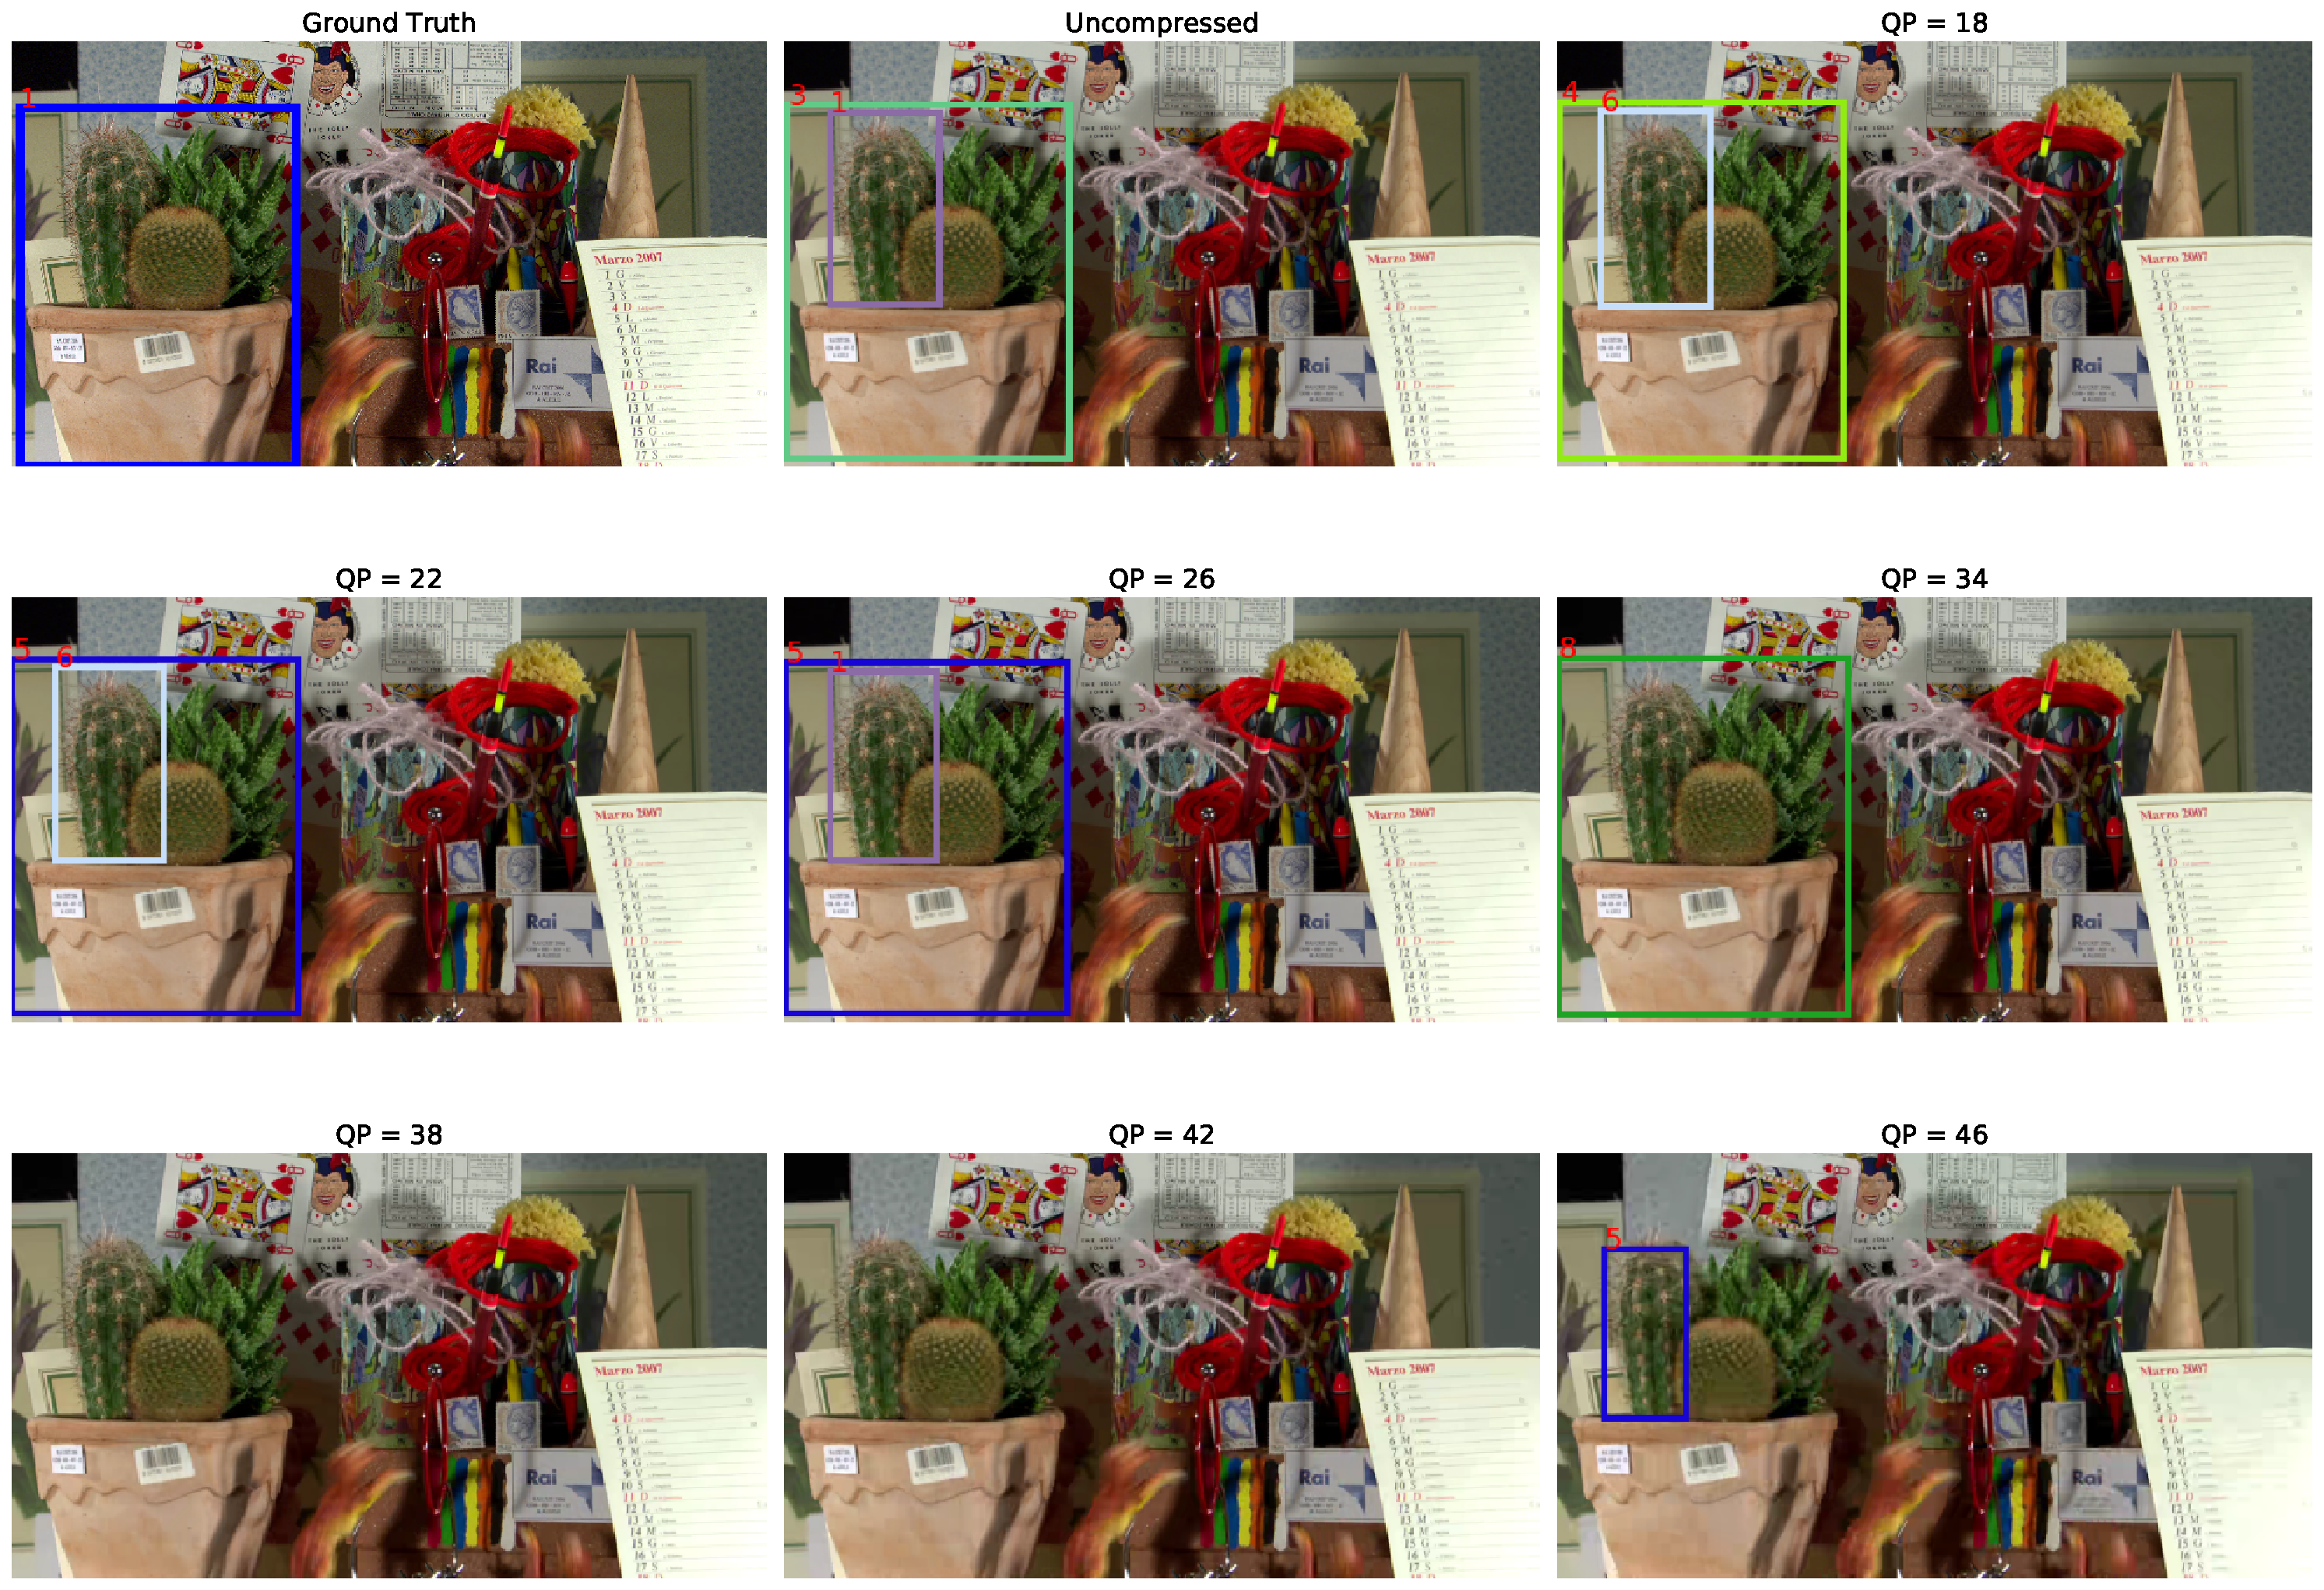
\includegraphics[width=1.0\linewidth]{img/Cactus_58_frame032.pdf}
  \caption[Comparison of Class B Cactus image frames at 32 among different QP]
  {
    Comparison of Class B Cactus image frames at 32 at different QP.
  }
  \label{fig:Cactus_58_frame032}
\end{figure}
From this comparison, we observed that YOLO v3 incorrectly detect two objects at a single target until QP = 26. Ground truth only contains 1 Potted plant. At QP = 34, we can see the correctly detected object at a single target but as QP increases further, the object is starting to not be detected and at QP = 46, YOLO v3 detected the wrong target. This proves the decrease of FP midway through the QP range but increase again at the high QP. It is also observed that FN decreases slightly at the middle of QP range but increases at the high QP since the correct target starts to not be detected. In fact, not only the case at frame 32, we also observed similar outcomes in the other frames. This reveals that the cause of an increase of MOTA midway through the range of QP is due to the decrease of FP and FN. The reason for the outcome we observed at the frame 32 as an example could be that the type of object is problematic in a way that 3 cactuses are in a vase, so YOLO v3 incorrectly detect one of cactuses as a potted plant instead of detecting the entire 3 cactuses in a vase as a potted plant.


\subsection{Discussion}
We inspected the 4 individual video sequences and focused on the general tracking performance of MOTA. From the inspected video samples, we found that MOTA performance scores in Class B BasketballPass and Class E Johnny are consistent with the hypothesis. However, the MOTA performance scores in Class D BlowingBubbles and Class B Cactus increase midway through the QP range and decrease thereafter. We found that these results are due to the type of object that makes the YOLO v3 detector incorrectly detect the wrong targets, and FP was observed to be high even at the uncompressed video. Recall that we are using SORT based on YOLO v3, a detection-based detector, so the tracking performance is dependent on the detection performance. Hence, the tracking performance is dependent on the ability of detector. This means that suppose we have a perfect detector, then we wouldn't be seeing such result of an increase of MOTA. Note that since FP was high at the uncompressed case, as QP increases and the image quality drops, FP was observed to be decreased. This insight also proves the reason why we observed an increase of Precision from the averaged result. From the equation \ref{eqn:Precision}, Precision depends on TP and FP and since FP decreases in some video samples, Precision was observed to be increased.

Not only the tracking performance that depends on the ability of the detector, it also depends on the ability of the tracker. Re-ID for the long term undetection is not implemented in our tracker, SORT, so it affects the ID measure and IDs.

Finally, for the MOTP metric, we observed an increase of MOTP in some sequences: Class D BasketballPass, Class E Johnny, and Class D BlowingBubbles. Since MOTP measures how well the objects are localized to the ground truth, the result from the individual sequences tells us that the object localization improves midway through the QP range but its localization performance decreases thereafter as the image quality further drops. Not all the video sequences behaves in this way but these outcomes contributed to the averaged result.